\chapter{Gradient Learning and Supervised Learning Techniques}

In the previous chapters ERM became an optimization problem: find the parameters that make the empirical risk as small as possible. This chapter first explains how this problem is solved in practice, with \textbf{gradient-based methods}, and how classification is extended to \textbf{more than two classes}. It then reviews the main \textbf{supervised learning techniques}, each described by the three design choices of ERM: data, model and loss.

When the hypothesis $h^{(\mathbf{w})}$ is described by a parameter vector $\mathbf{w} \in \mathbb{R}^n$, ERM is the problem
\[
\min_{\mathbf{w} \in \mathbb{R}^n} f(\mathbf{w}) := \frac{1}{m}\sum_{i=1}^{m} \underbrace{L\big((\mathbf{x}^{(i)}, y^{(i)}), h^{(\mathbf{w})}\big)}_{f_i(\mathbf{w})} .
\]
Here $f_i(\mathbf{w})$ is the loss of the hypothesis on the $i$-th training point and $f(\mathbf{w})$, the empirical risk, is the average of the $m$ single losses. If each single loss $f_i(\mathbf{w})$ is differentiable, $f(\mathbf{w})$ is also differentiable, and we can use its derivatives to find the minimum. For linear regression the minimum can even be computed with a formula, but for most models no formula exists and an iterative method is needed.

\section{Gradient Based Methods}
Gradient Based Methods are iterative: they construct a sequence of parameter vectors $\mathbf{w}^{(0)} \rightarrow \mathbf{w}^{(1)} \rightarrow \dots$ that hopefully converges to the minimum of $f(\mathbf{w})$. The intuition is that of a hiker in the fog who wants to reach the bottom of a valley: she cannot see the valley, but she can feel the slope of the ground under her feet, so she takes a step downhill, then another one.

\subsection{Gradient Descent}
The slope is given by the \textbf{gradient} $\nabla f(\mathbf{w})$, the vector of the partial derivatives $\partial f/\partial w_1, \dots, \partial f/\partial w_n$. It points in the direction in which $f$ grows fastest, and its length says how steep $f$ is. The gradient allows to locally approximate $f(\mathbf{w})$ with a linear function, the tangent line (or tangent plane) at the point we are considering:\footnote{Correction: the previous version defined the gradient as ``the tangent line to the point we are locally considering''. The gradient is the vector of partial derivatives; the tangent line (or plane) is the linear approximation built with it.}
\[
f(\mathbf{w}) \approx f(\mathbf{w}^{(r)}) + (\mathbf{w} - \mathbf{w}^{(r)})^{T}\, \nabla f(\mathbf{w}^{(r)}) \qquad \text{for } \mathbf{w} \text{ sufficiently close to } \mathbf{w}^{(r)} .
\]
The first term is the current value of the empirical risk; the second term says how much it changes when we move from $\mathbf{w}^{(r)}$ to $\mathbf{w}$. Since we want to minimize $f(\mathbf{w})$, we should move in a direction such that the second term is negative, and it is most negative when we move \textbf{opposite to the gradient}. Given the current guess $\mathbf{w}^{(r)}$, the next guess is
\[
\mathbf{w}^{(r+1)} = \mathbf{w}^{(r)} - \alpha\, \nabla f(\mathbf{w}^{(r)}) \qquad \text{with a sufficiently small step size } \alpha > 0 .
\]
This is the \textbf{gradient descent (GD) step}, and $\alpha$ is the \textbf{learning rate}: it sets the width of the step taken to follow the decreasing direction.\footnote{Correction: the previous version defined the gradient descent step as ``the width of the local steps''. The step is the whole update $\mathbf{w}^{(r+1)} = \mathbf{w}^{(r)} - \alpha\nabla f(\mathbf{w}^{(r)})$; its width is controlled by the learning rate $\alpha$ (and by the steepness $\|\nabla f\|$).} Where $f$ is steep the step is long; near the minimum, where $f$ is flat, the steps become short.

\begin{figure}[h]
    \centering
    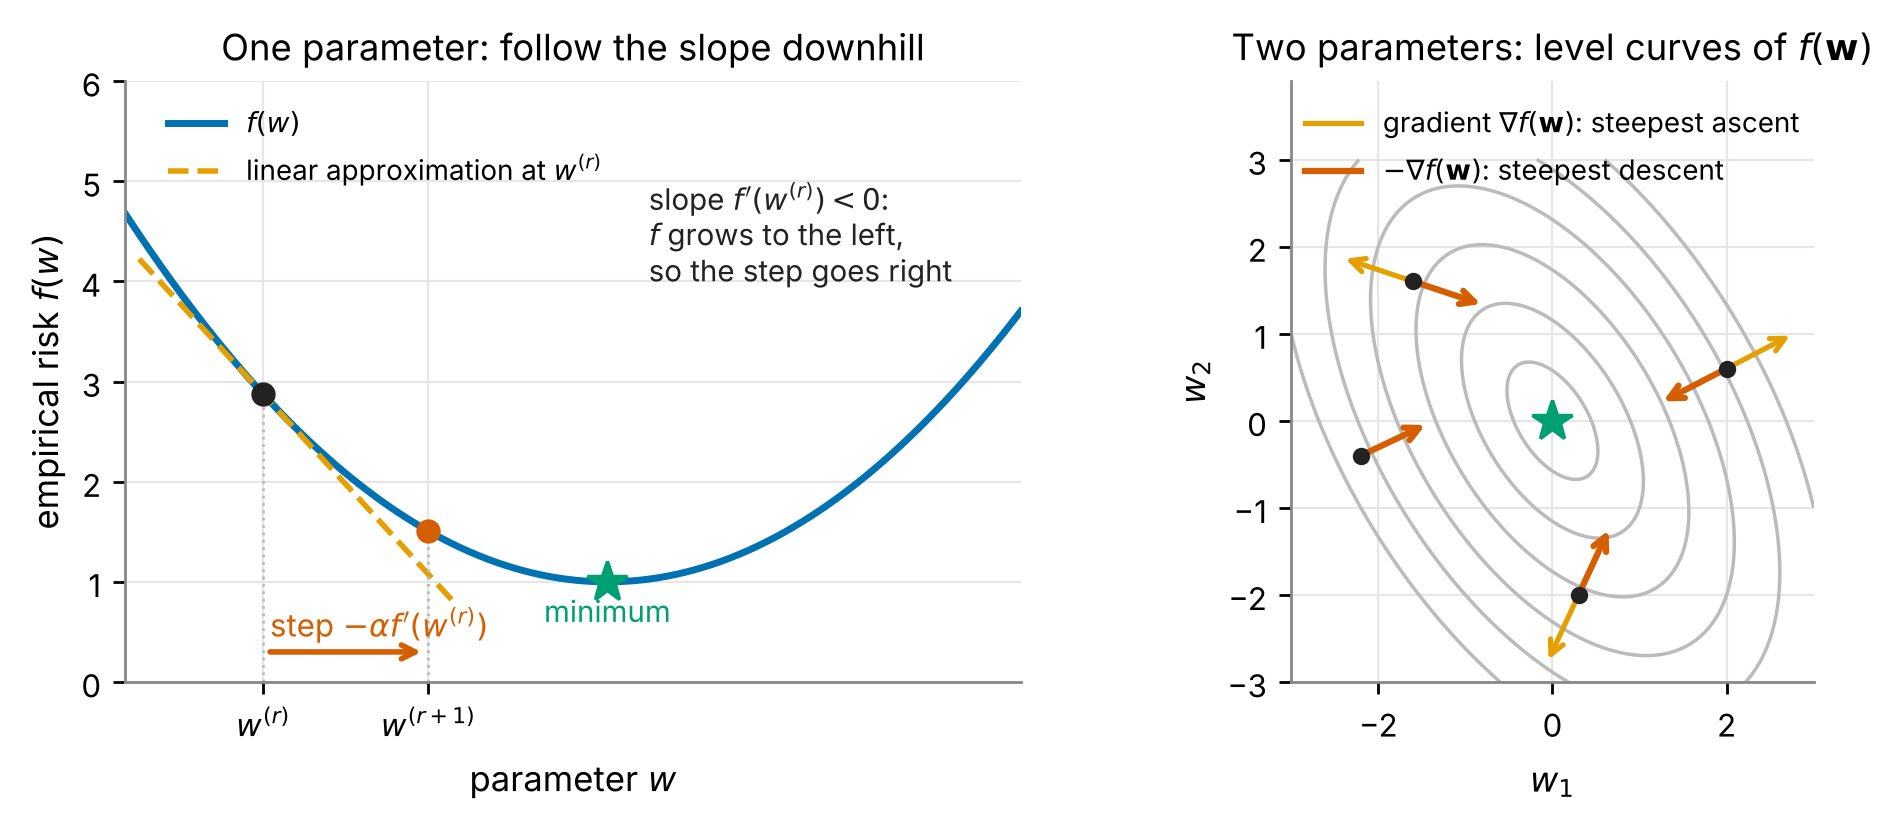
\includegraphics[width=1\textwidth]{images/chapter_9/gd_step.png}
    \caption{Left: one GD step with one parameter; the linear approximation (dashed) tells in which direction $f$ decreases. Right: with two parameters the gradient is perpendicular to the level curves of $f$ and points uphill; GD moves the other way.}
\end{figure}

For example, take $f(w) = w^2$, whose derivative is $f'(w) = 2w$, start from $w^{(0)} = -4$ and use $\alpha = 0.35$. Then $w^{(1)} = -4 - 0.35 \cdot (-8) = -1.2$, $w^{(2)} = -1.2 - 0.35 \cdot (-2.4) = -0.36$, and so on: each step multiplies $w$ by $1 - 2\alpha = 0.3$, and after a few steps we are at the minimum $w = 0$.

\begin{center}
\fbox{\parbox{0.9\textwidth}{
\textbf{Algorithm: gradient descent}\\
\textbf{Input:} training set, loss $L$, learning rate $\alpha$, stopping criterion\\
\textbf{Output:} parameter vector $\mathbf{w}$
\begin{enumerate}
    \item Initialize $\mathbf{w}^{(0)}$ (e.g. all zeros, or random) and set $r = 0$.
    \item Compute the gradient $\nabla f(\mathbf{w}^{(r)}) = \frac{1}{m}\sum_{i=1}^{m} \nabla f_i(\mathbf{w}^{(r)})$.
    \item Update $\mathbf{w}^{(r+1)} = \mathbf{w}^{(r)} - \alpha\,\nabla f(\mathbf{w}^{(r)})$ and set $r \leftarrow r + 1$.
    \item If the stopping criterion is met return $\mathbf{w}^{(r)}$, otherwise go back to step 2.
\end{enumerate}}}
\end{center}

\subsection{Choosing the Learning Rate}
Choosing the learning rate is crucial. If $\alpha$ is too small, the steps are tiny and GD needs a huge number of iterations; if it is too large, each step jumps over the minimum to the other side of the valley, and GD oscillates or even diverges. In the example $f(w) = w^2$ each step multiplies $w$ by $1 - 2\alpha$, so GD converges only for $0 < \alpha < 1$: after 5 steps from $w^{(0)} = -4$, $\alpha = 0.05$ is still at $f = 5.58$, $\alpha = 0.35$ is practically at the minimum, while with $\alpha = 1.05$ the value of $|w|$ grows by 10\% at each step and $f$ reaches $41.5$.

\begin{figure}[h]
    \centering
    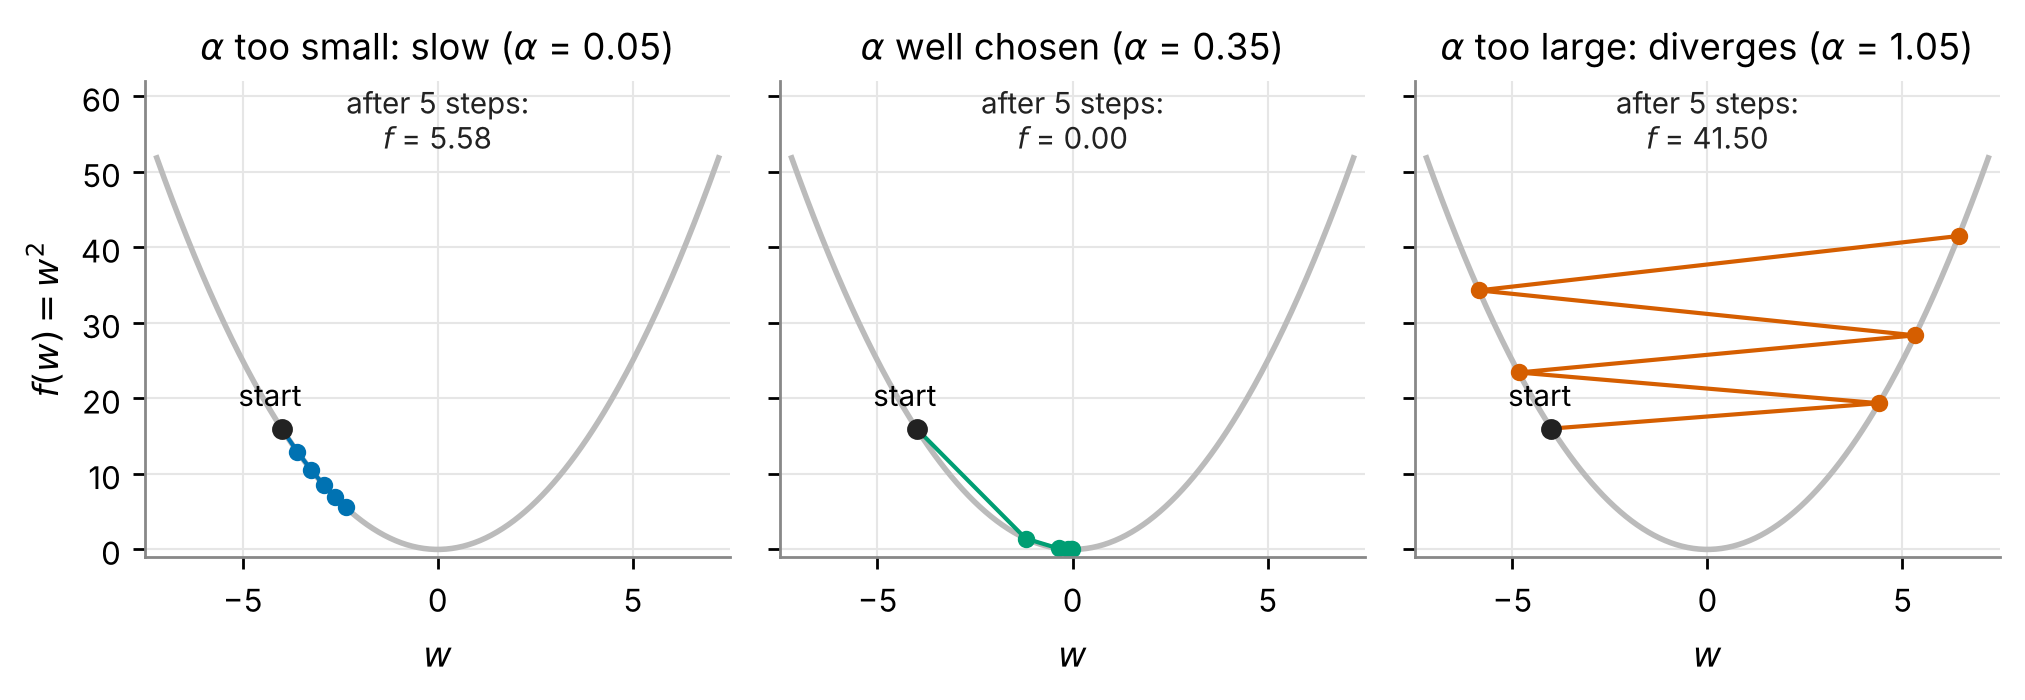
\includegraphics[width=1\textwidth]{images/chapter_9/learning_rate.png}
    \caption{Five GD steps on $f(w) = w^2$ from $w^{(0)} = -4$ with three learning rates.}
\end{figure}

In some cases theoretical bounds and optimal values for $\alpha$ can be given; for the squared error loss of linear regression, for instance, they depend only on the feature vectors of the training set. In practice $\alpha$ is often treated as a hyper-parameter: we try a few values (e.g. $0.001$, $0.01$, $0.1$) and keep the one for which the empirical risk decreases fastest without oscillating.

The general rule is that GD needs fewer steps on \textbf{standardized data}, hence it is better to standardize the features at the beginning (see the Data Pre-processing chapter). If one feature is measured in bytes and another in seconds, the empirical risk is a long and narrow valley: $f$ is very steep in one direction and almost flat in the other. The learning rate must be small enough for the steep direction, so the progress along the flat direction is slow, and the path zig-zags from one side of the valley to the other. After standardization the valley is much rounder and the path goes almost straight to the minimum.

\begin{figure}[h]
    \centering
    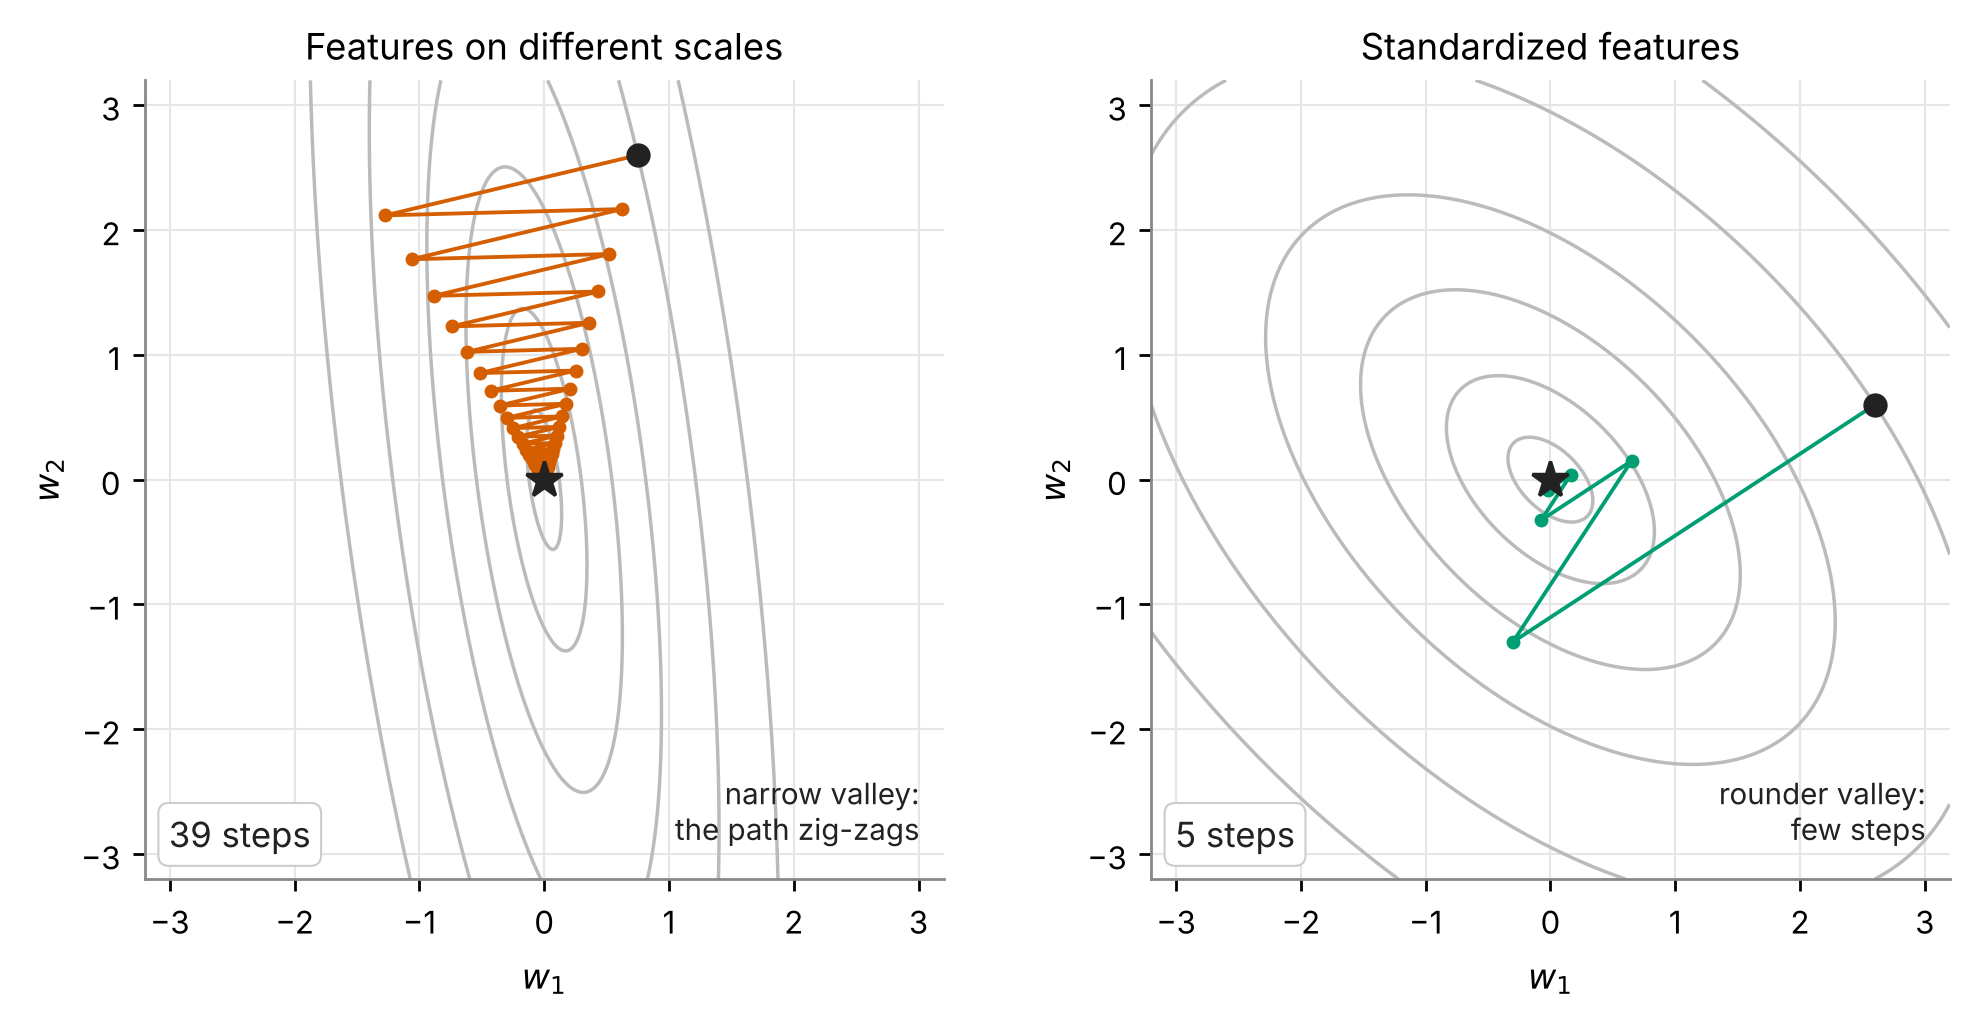
\includegraphics[width=1\textwidth]{images/chapter_9/standardization.png}
    \caption{GD with the best fixed learning rate on the same problem, before and after standardizing the features: 39 steps against 5 to reduce the empirical risk to 0.1\% of its initial value.}
\end{figure}

\subsection{Stopping Criteria}
Additionally, there are different strategies to define when to stop the GD steps:
\begin{itemize}
    \item \textbf{Fixed number of iterations}. One pass over the whole training set is called an \textbf{epoch}; in plain GD every iteration uses all the training points, so one iteration is one epoch.
    \item When the difference between the empirical risk at the previous step and at this step is less than a threshold, meaning that the empirical risk is not improving anymore.
    \item When the validation error stops decreasing (\textbf{early stopping}).\footnote{Correction: the previous version said to stop ``when validation error keep decreasing''. As long as the validation error decreases the model is still improving on new data; we stop when it stops decreasing and starts to grow.}
\end{itemize}

\begin{figure}[h]
    \centering
    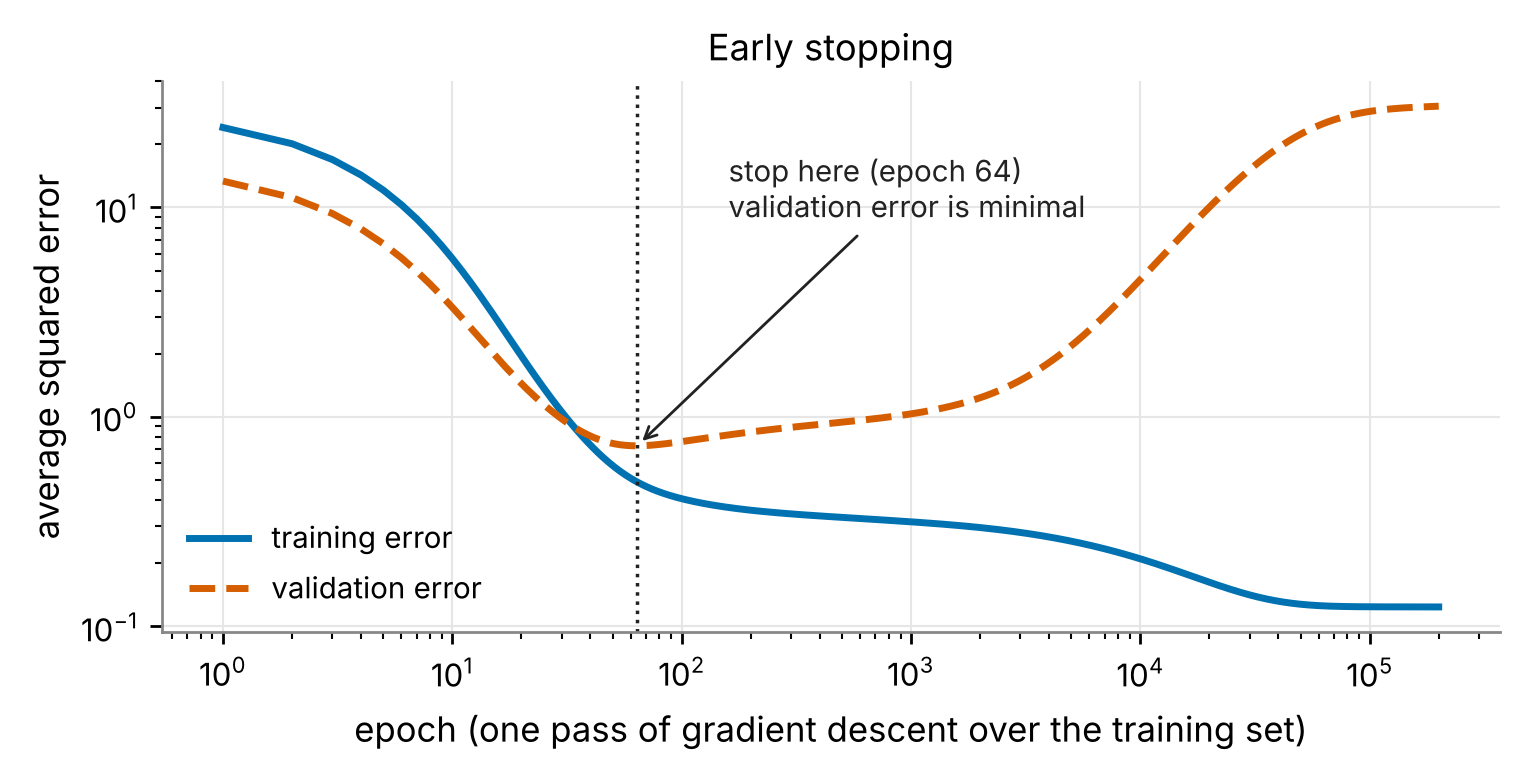
\includegraphics[width=0.8\textwidth]{images/chapter_9/early_stopping.png}
    \caption{GD on a polynomial of degree 15 learnt from 20 measurements of the queueing delay of a link (both axes in log scale).}
\end{figure}

Early stopping protects against overfitting. In the figure a very flexible model (a polynomial with 16 coefficients) is learnt by GD from only 20 training points. The validation error is minimal at epoch 64 ($0.73$); if we keep going until epoch 200\,000, the training error decreases to $0.12$ but the validation error grows to $30.5$, because the model is learning the noise of the training points. In practice we wait a few epochs before stopping (a ``patience''), because the validation error fluctuates, and we keep the parameters of the best epoch.

\subsection{Stochastic Gradient Descent}
Computing the gradient $\nabla f(\mathbf{w}) = \frac{1}{m}\sum_{i} \nabla f_i(\mathbf{w})$ requires a pass over all the $m$ training points at every step, and this is challenging for large $m$, e.g. millions of flow records. \textbf{Stochastic Gradient Descent} (SGD) computes an approximation of the gradient instead:
\begin{enumerate}
    \item Iteratively replace the sum with a random component: pick a random index $i_r$ and use $\nabla f_{i_r}$ in place of $\nabla f$, i.e. $\mathbf{w}^{(r+1)} = \mathbf{w}^{(r)} - \alpha\,\nabla f_{i_r}(\mathbf{w}^{(r)})$.
    \item Iteratively replace the sum with a random \textbf{batch} $\mathcal{B} = \{i_1, \dots, i_B\}$ of $B$ indices (\textbf{mini-batch SGD}), and use
    \[
    g(\mathbf{w}) = \frac{1}{B}\sum_{i' \in \mathcal{B}} \nabla f_{i'}(\mathbf{w}) .
    \]
\end{enumerate}
In this case the real gradient is approximated by the \textbf{average} of the gradients of the randomly selected subset, the batch.\footnote{Correction: the previous version said that the gradient is approximated by ``the sum'' of the selected subset. It is the average, $\frac{1}{B}\sum_{i' \in \mathcal{B}}\nabla f_{i'}$, which has the same scale as the true gradient; it is like estimating the mean of a population from a random sample.} On average the approximation equals the true gradient, but it is noisy: the path zig-zags and, with a constant learning rate, keeps fluctuating around the minimum. A larger batch, or a learning rate that decreases over time, reduces the noise.

\begin{figure}[h]
    \centering
    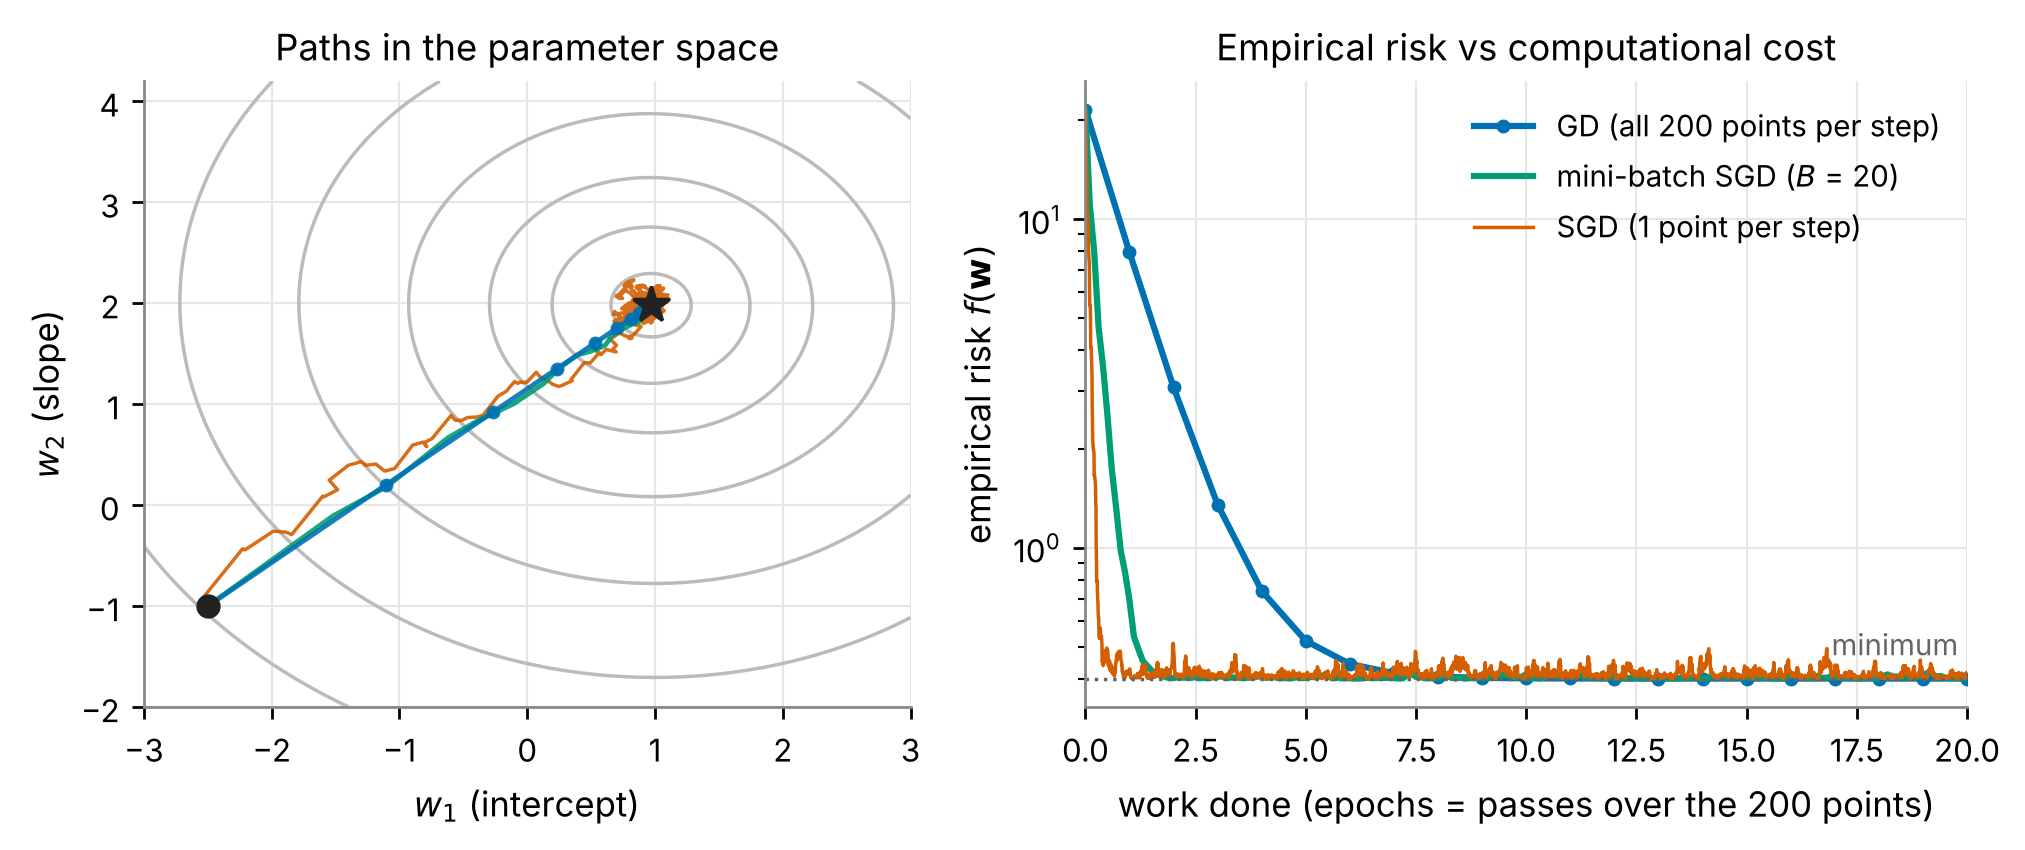
\includegraphics[width=1\textwidth]{images/chapter_9/sgd.png}
    \caption{Linear regression on 200 points with GD, mini-batch SGD and SGD. Right: empirical risk against the work done, measured in epochs (one epoch = one GD step = 10 mini-batch steps = 200 SGD steps).}
\end{figure}

The advantage is speed: with the same work as \emph{one} GD step, SGD makes 200 small steps. In the figure, after one epoch the empirical risk is $7.91$ with GD, $0.69$ with mini-batch SGD and $0.42$ with SGD, against a minimum of $0.40$. SGD is also the natural choice for \textbf{online learning}, e.g. a traffic model that is updated with every new batch of flow records instead of being retrained from scratch.

\begin{center}
    \begin{tabular}{l|c|c|l}
        & \textbf{Points/step} & \textbf{Steps/epoch} & \textbf{Path} \\ \hline
        GD             & $m$ & $1$   & smooth, costly steps \\
        Mini-batch SGD & $B$ & $m/B$ & a bit noisy: usual choice \\
        SGD            & $1$ & $m$   & noisy, very cheap steps \\
    \end{tabular}
\end{center}

\section{Multi-class and Multi-label Classification}
So far classification was binary, $y \in \{-1, +1\}$. There are two different extensions:
\begin{itemize}
    \item \textbf{multi-class}: one label with more than two possible values, e.g. the application of a flow, $y \in \{\text{web}, \text{video}, \text{VoIP}\}$;
    \item \textbf{multi-label}: several labels for each data point, e.g. the application of a flow \emph{and} whether it is encrypted.
\end{itemize}
In order to perform multi-class classification it is possible to use the one-vs-rest trick or, for logistic regression, the softmax; the naive and the combination approaches are used for multi-label classification.\footnote{Correction: the previous version listed the one-vs-rest trick, the naive approach and the ``each combination is a new category'' approach all as multi-class techniques. The last two make sense only when there are several labels per data point, i.e. for multi-label classification.}

\subsection{One-vs-Rest}
The \textbf{one-vs-rest} trick divides the classification into $n_{\text{labels}}$ binary classification problems, where $n_{\text{labels}}$ is the number of label values: problem 1 has label value 1 against all the remaining classes, and so on. We produce one sub-problem for each label value $c$, where the sub-problem $c$ is: \emph{label $= c$ or not}. Each binary classifier returns a score $h_c(\mathbf{x})$, its confidence that $\mathbf{x}$ belongs to class $c$, and the final prediction is the class with the \textbf{largest score}. For example, if a flow gets the scores $+1.2$ (web vs rest), $-0.5$ (video vs rest) and $-2.0$ (VoIP vs rest), it is classified as web.

\begin{figure}[h]
    \centering
    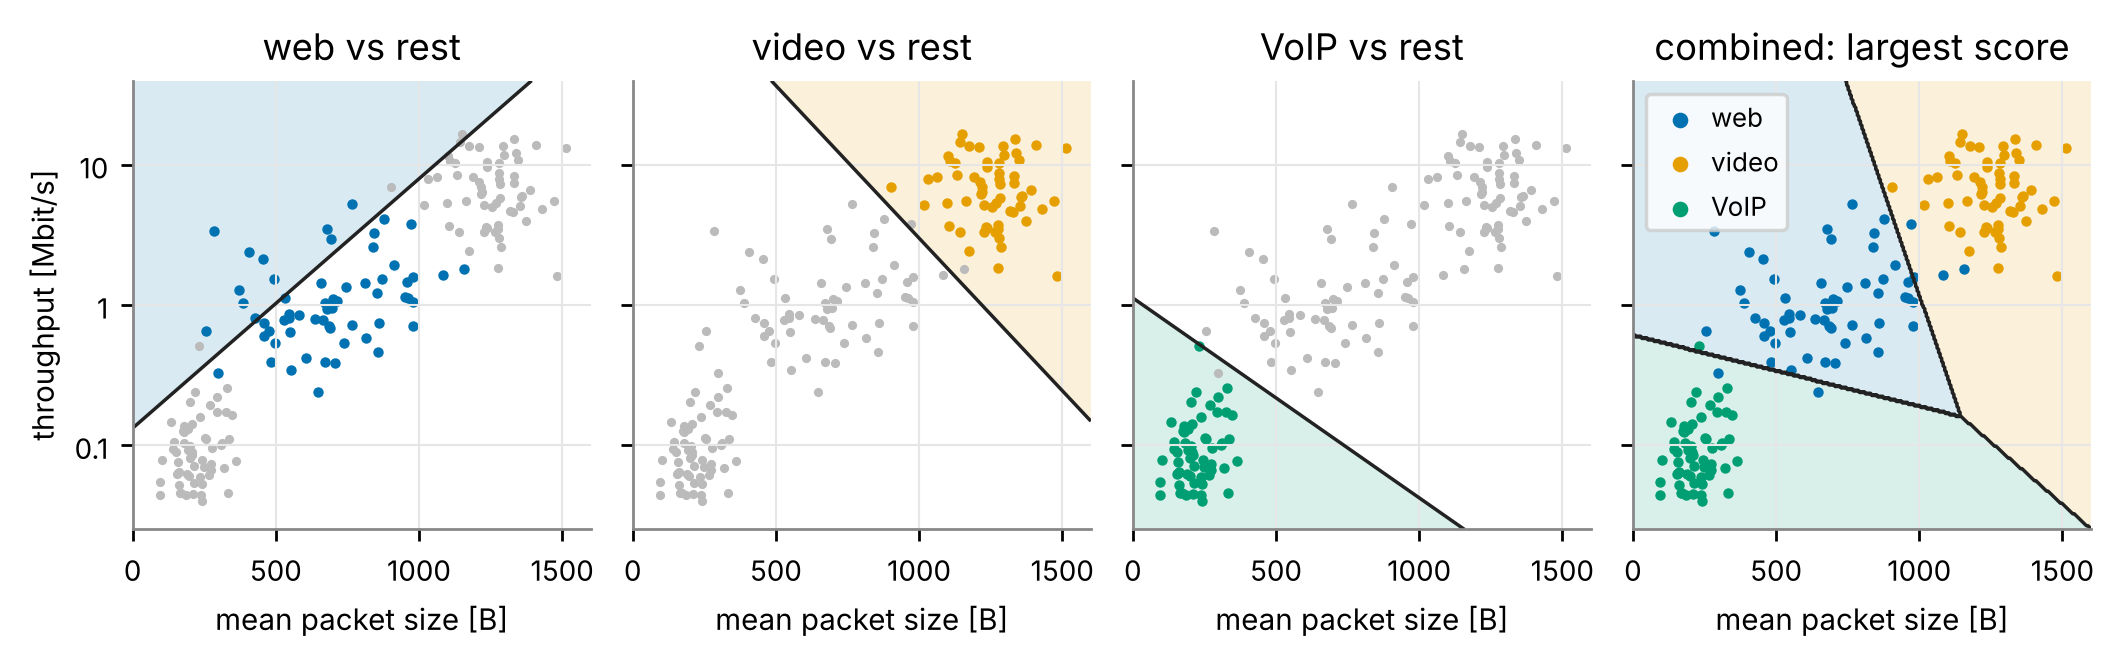
\includegraphics[width=1\textwidth]{images/chapter_9/one_vs_rest.png}
    \caption{One-vs-rest with logistic regression on 180 flows of three applications: three binary problems, combined by choosing the largest score (training accuracy 0.96).}
\end{figure}

\subsection{Softmax}
Lastly, for multi-class problems logistic regression defines the confidence of the prediction thanks to the \textbf{softmax}. The model computes one score $h_c(\mathbf{x}) = \mathbf{w}_c^{T}\mathbf{x}$ for each of the $k$ classes, and the softmax turns the scores into probabilities:
\[
p_c(\mathbf{x}) = \frac{\exp\big(h_c(\mathbf{x})\big)}{\sum_{c'=1}^{k}\exp\big(h_{c'}(\mathbf{x})\big)} .
\]
Each $p_c(\mathbf{x})$ is between 0 and 1, they sum to 1, and the class with the largest score gets the largest probability. The loss is $L = -\log p_y(\mathbf{x})$, the negative logarithm of the probability given to the \emph{true} class $y$ (\textbf{cross-entropy}). It extends the logistic loss to $k$ classes: for $k = 2$ it is exactly the logistic loss. It is a smooth loss: it is close to 0 when the true class gets a probability close to 1, and it grows without limit when the true class gets a probability close to 0, i.e. when the classifier is confident and wrong.\footnote{Correction: the previous version said that the softmax extends the logistic loss ``not anymore a 0/1 loss for only 1 classes''. The softmax extends the \emph{logistic} loss (not the 0/1 loss) from 2 to $k$ classes; the loss is $-\log$ of the probability of the true class.}

\begin{figure}[h]
    \centering
    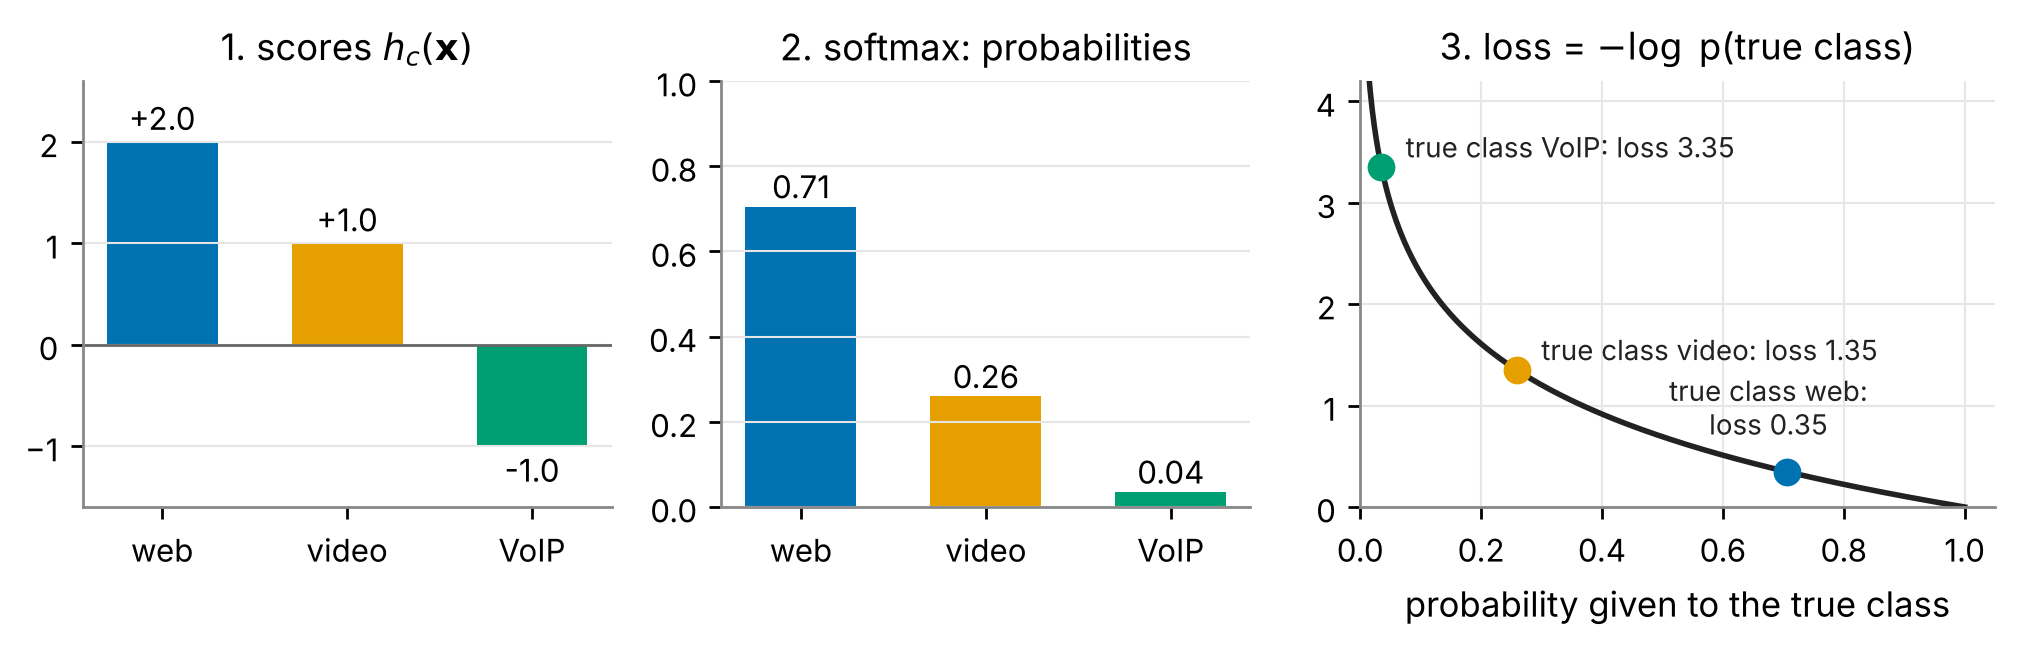
\includegraphics[width=1\textwidth]{images/chapter_9/softmax.png}
    \caption{From scores to probabilities to loss, for a flow with scores $2$, $1$ and $-1$.}
\end{figure}

For example, the scores $2$, $1$, $-1$ give $\exp(2) = 7.39$, $\exp(1) = 2.72$, $\exp(-1) = 0.37$, whose sum is $10.48$, hence the probabilities $0.71$, $0.26$ and $0.04$. If the flow is really web the loss is $-\log 0.71 = 0.35$; if it is VoIP, the class the model considered least likely, the loss is $-\log 0.035 = 3.35$.

\subsection{Multi-label Classification}
With several labels per data point there are two approaches:
\begin{itemize}
    \item \textbf{Naive approach}: consider each label separately and solve a (binary or multi-class) problem for each label: one classifier for the application, one for encrypted yes/no. It is simple, but it ignores the correlations between the labels.
    \item \textbf{Combination approach}: each combination of label values defines a new category, and a single multi-class problem is solved. With 3 applications and encrypted yes/no we get $3 \times 2 = 6$ classes. Correlations are captured, but the number of classes is the product of the numbers of label values, so it grows quickly and some combinations have very few examples.
\end{itemize}

\section{Supervised Learning Techniques}
It is useful to differentiate the Supervised Learning Techniques for regression and classification tasks. Several of them can be used for both.

\begin{center}
    \begin{tabular}{l|l}
        \textbf{Regression} & \textbf{Classification} \\ \hline
        Linear and polynomial regression & Logistic regression \\
        LASSO regressor & Support Vector Machines \\
        Decision tree and random forest & Naive Bayes classifier \\
        k-Nearest Neighbors & Decision tree and random forest \\
        Neural networks and deep learning & k-Nearest Neighbors \\
        & Neural networks and deep learning \\
    \end{tabular}
\end{center}
Neural networks are covered in the next chapters. For each of the other techniques we give the three design choices of ERM: data, model and loss.

\subsection{LASSO Regressor}
The \textbf{LASSO} regressor, which stands for least absolute shrinkage and selection operator, is a supervised regressor with the following characteristics:
\begin{itemize}
    \item \textbf{DATA}: numeric features and label;
    \item \textbf{MODEL}: space of linear maps;
    \item \textbf{LOSS}: regularized squared loss,
\end{itemize}
\[
L\big((\mathbf{x}, y), h^{(\mathbf{w})}\big) = \big(y - \mathbf{w}^{T}\mathbf{x}\big)^2 + \lambda \|\mathbf{w}\|_1, \qquad \|\mathbf{w}\|_1 = |w_1| + |w_2| + \dots + |w_n| .
\]
It is useful to remember that ordinary linear regression requires the training set to be larger than the number of features ($m > n$) to avoid \textbf{overfitting}: with $m \leq n$ there are infinitely many weight vectors that fit the training points exactly. However, often $m < n$, e.g. hundreds of traffic statistics measured on a few dozen labelled incidents. LASSO, thanks to the penalty, can be used also when $m < n$.\footnote{Correction: the previous version said that LASSO, since it solves a linear regression problem, requires $m > n$. It is plain linear regression that needs $m > n$; the penalty of LASSO is what allows it to work also when $m < n$.}

The \textbf{regularization technique} adds to the loss a penalty, weighted by $\lambda \geq 0$, for using too many features. In a nutshell, the loss function has 2 components:
\begin{itemize}
    \item \textbf{first component}: the squared loss, which asks the model to fit the training data;
    \item \textbf{penalty} $\lambda\|\mathbf{w}\|_1$: a larger penalty favours simpler models using fewer features, by setting more coefficients exactly to 0. It works as \textbf{feature selection}.
\end{itemize}
By increasing $\lambda$, the weight vector $\mathbf{w}$ has more and more zero coefficients. Why exactly zero? The weights that minimize the loss sit where the level curves of the squared error first touch a ``ball'' $\|\mathbf{w}\|_1 \leq t$. For $\|\cdot\|_1$ the ball is a diamond with corners on the axes, and the contact typically happens at a corner, where some weights are exactly 0. \textbf{Ridge regression} uses the penalty $\lambda\|\mathbf{w}\|_2^2$ instead, whose ball is round: it shrinks the weights but almost never makes them zero.

\begin{figure}[h]
    \centering
    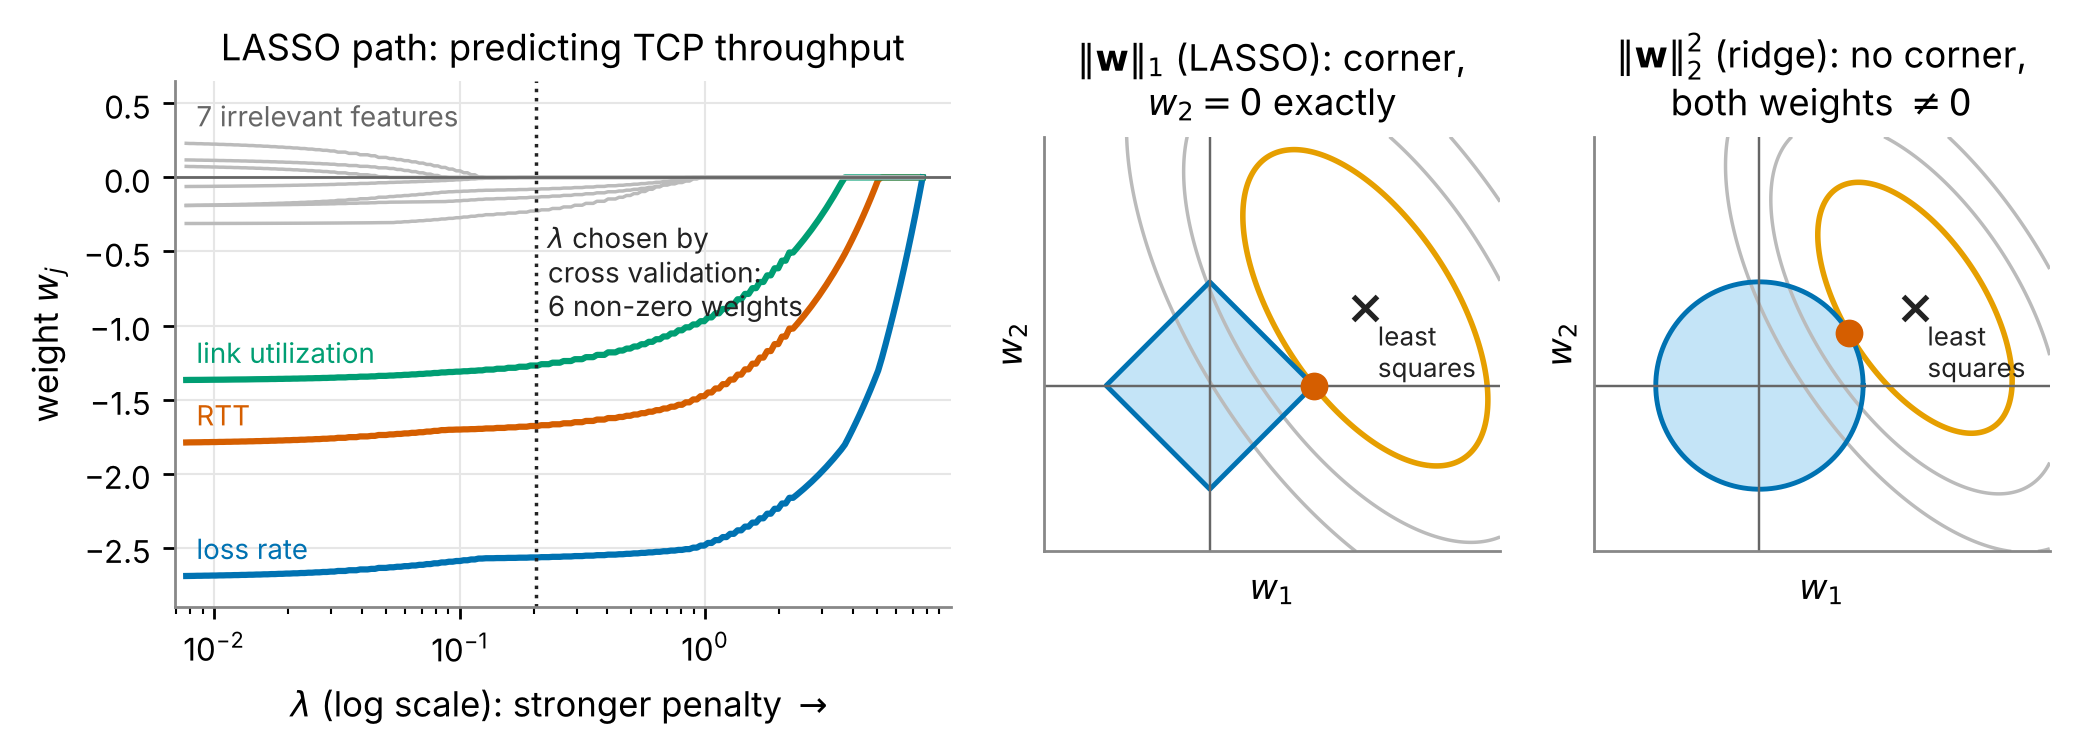
\includegraphics[width=1\textwidth]{images/chapter_9/lasso.png}
    \caption{Left: LASSO weights for predicting the throughput of a TCP connection from 10 standardized features measured on 40 connections, as $\lambda$ grows. Right: why the L1 penalty produces exact zeros while the L2 penalty does not.}
\end{figure}

In the figure only 3 of the 10 features really influence the throughput (RTT, loss rate and link utilization). As $\lambda$ grows all weights shrink, and the irrelevant ones reach 0 first. The $\lambda$ chosen by cross validation keeps 6 non-zero weights: the 3 relevant features with large weights, and 3 irrelevant ones with small weights (below $0.25$ in absolute value), while hop count, packet size, hour of day and window size get exactly 0. A larger $\lambda$ keeps only the relevant features; a very large one sets all weights to 0, and the model predicts the mean throughput. $\lambda$ is a hyper-parameter, chosen with a validation curve or cross validation; the features must be standardized, otherwise the penalty would depend on their units.

\subsection{Support Vector Machines}
The \textbf{SVM}, or Support Vector Machine, is a supervised classifier used to perform linear classification:
\begin{itemize}
    \item \textbf{DATA}: numeric features, binary label values $y \in \{-1, +1\}$;
    \item \textbf{MODEL}: space of linear maps;
    \item \textbf{LOSS}: regularized hinge loss.
\end{itemize}
SVM and logistic regression share the same data and model and differ only in the loss: replacing the hinge loss with the logistic loss turns the SVM into logistic regression.\footnote{Clarification: the previous version said that the SVM ``can be also used for logistic regression tasks, by changing the loss function''. With a different loss it is no longer an SVM: the point is that the two methods are two instances of ERM that differ only in the loss.}

SVM looks for a hyperplane, the decision boundary, that separates the data. It needs a \textbf{regularized} hinge loss because, for a linearly separable dataset, there might be infinitely many linear maps with 0 average hinge loss: any separating line, with large enough weights, classifies every point correctly with confidence $y\,h(\mathbf{x}) \geq 1$. The regularized hinge loss used in SVM is
\[
\frac{1}{m}\sum_{i=1}^{m} \max\big(0,\ 1 - y^{(i)} h^{(\mathbf{w})}(\mathbf{x}^{(i)})\big) + \lambda\|\mathbf{w}\|_2^2 .
\]
\begin{itemize}
    \item \textbf{First member}: the average hinge loss, zero for the points classified correctly with enough confidence.
    \item \textbf{Second member}: the regularization, weighted by $\lambda$, which penalizes large weights in order to \textbf{maximize the margin}, i.e. the distance between the decision boundary and the closest training points. The width of the margin is $2/\|\mathbf{w}\|_2$, so smaller weights mean a wider margin.
\end{itemize}
The end goal is a decision boundary that separates the data and maximizes the margin: among all the separating lines, the SVM picks the safest one, the farthest from both classes, which increases the confidence of the classification. A new point slightly different from the training points is still on the right side.

\begin{figure}[h]
    \centering
    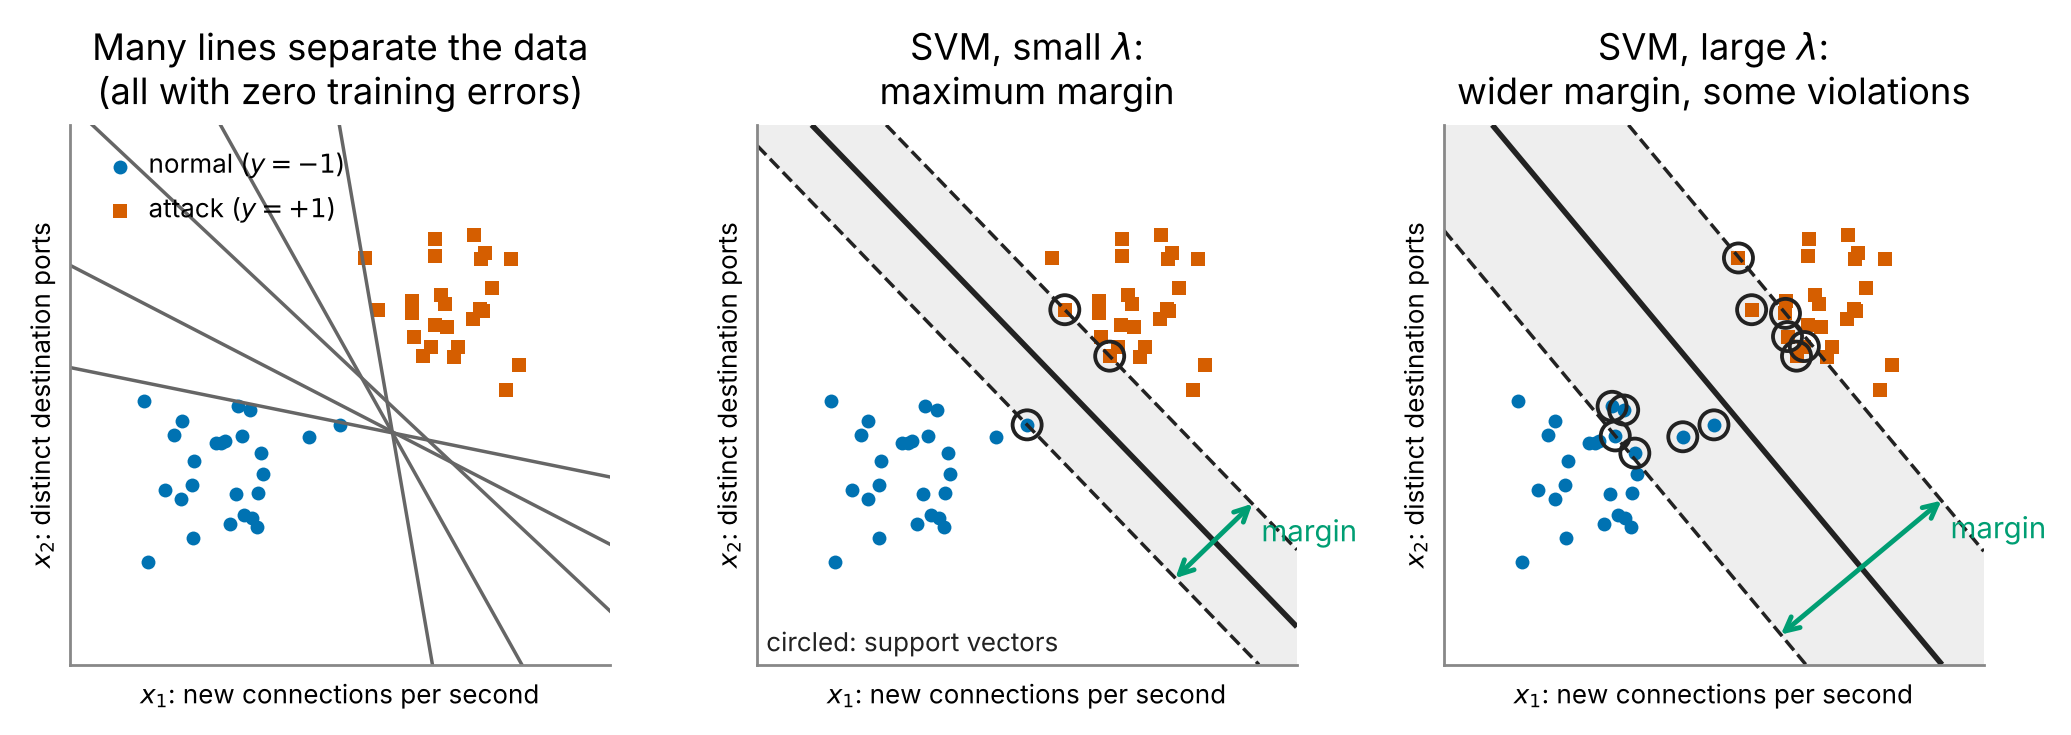
\includegraphics[width=1\textwidth]{images/chapter_9/svm.png}
    \caption{Detecting port scans from the number of new connections per second and of distinct destination ports. Left: many lines separate the classes. Centre and right: the SVM boundary (solid) and margin (dashed) for a small and a large $\lambda$.}
\end{figure}

The parameter $\lambda$ sets the trade-off. With a small $\lambda$ the hinge loss dominates and no point may fall inside the margin (\textbf{hard margin}, width $1.19$ in the figure). With a large $\lambda$ the margin becomes wider ($2.33$) and some points are allowed inside it (\textbf{soft margin}), which makes the SVM more robust to noisy points. The points on or inside the margin are the \textbf{support vectors}: they alone determine the boundary, and moving any other point does not change it. In scikit-learn the trade-off is set by the parameter $C$, which plays the role of $1/\lambda$: a large $C$ means a small $\lambda$. With the so-called kernel trick, SVMs can also learn non-linear boundaries.

\subsection{Naive Bayes Classifier}
The \textbf{Naive Bayes} classifier is a supervised classifier that works with the following design choices:
\begin{itemize}
    \item \textbf{DATA}: numeric features, binary labels;
    \item \textbf{MODEL}: space of linear maps;\footnote{Note: the decision boundary of Gaussian Naive Bayes is linear only when each feature has the same variance in the two classes; when the variances depend on the class, as described below, the boundary is a curve (quadratic). This is probably a simplification of the course, so it is kept here; the figure shows both cases.}
    \item \textbf{LOSS}: 0/1 loss.
\end{itemize}
The 0/1 loss counts the errors, which is exactly what we care about, but it is flat almost everywhere and cannot be minimized with gradient methods (see the Empirical Risk chapter). Naive Bayes takes another route. The hypothesis that minimizes the expected 0/1 loss is known, the \textbf{Bayes classifier}: given the features $\mathbf{x}$, classify the sample as the class $y$ with maximum $p(y\,|\,\mathbf{x})$. In the binary case
\[
\widehat{h}(\mathbf{x}) =
\begin{cases}
1 & \text{if } p(y = 1\,|\,\mathbf{x}) > p(y = -1\,|\,\mathbf{x}) \\
-1 & \text{otherwise.}
\end{cases}
\]
In a nutshell, if, given the features $\mathbf{x}$, the probability of class $1$ is higher than the probability of class $-1$, $\mathbf{x}$ is classified as class $1$. The problem is that we do not have this probability distribution.

The Naive Bayes classifier estimates it from the training points, using Bayes' theorem $p(y\,|\,\mathbf{x}) = p(\mathbf{x}\,|\,y)\,p(y)/p(\mathbf{x})$:
\begin{itemize}
    \item $p(\mathbf{x})$ is the same for all $y$, so it does not affect the comparison and can be ignored;
    \item $p(y)$, the probability of class $y$, is estimated by the relative frequency of class $y$ in the training set;
    \item $p(\mathbf{x}\,|\,y)$ is estimated with the \textbf{naive hypothesis}: the features are independent given the class, so $p(\mathbf{x}\,|\,y) = p(x_1\,|\,y) \cdot p(x_2\,|\,y) \cdots p(x_n\,|\,y)$, and each $x_j$ is a one-dimensional Gaussian random variable with mean and variance depending on $y$ (the sample mean and variance of feature $j$ over the training points of class $y$).
\end{itemize}
Therefore we have two Gaussian distributions for each feature, one for the positive class and one for the negative class. Their product gives two distributions over the whole feature vector, one per class, and the decision boundary separates the regions where $p(\mathbf{x}\,|\,1)\,p(1)$ or $p(\mathbf{x}\,|\,{-1})\,p(-1)$ is larger. Training does not solve an optimization problem: it only computes frequencies, means and variances, which are then plugged into the Bayes classifier.\footnote{Correction: the previous version said that Naive Bayes ``tries to minimize the ERM by computing the single probabilities''. Naive Bayes does not minimize the empirical risk: it estimates a probability model from the training data and then applies the Bayes classifier, which would minimize the expected 0/1 loss if the estimated probabilities were exact.}

\begin{figure}[h]
    \centering
    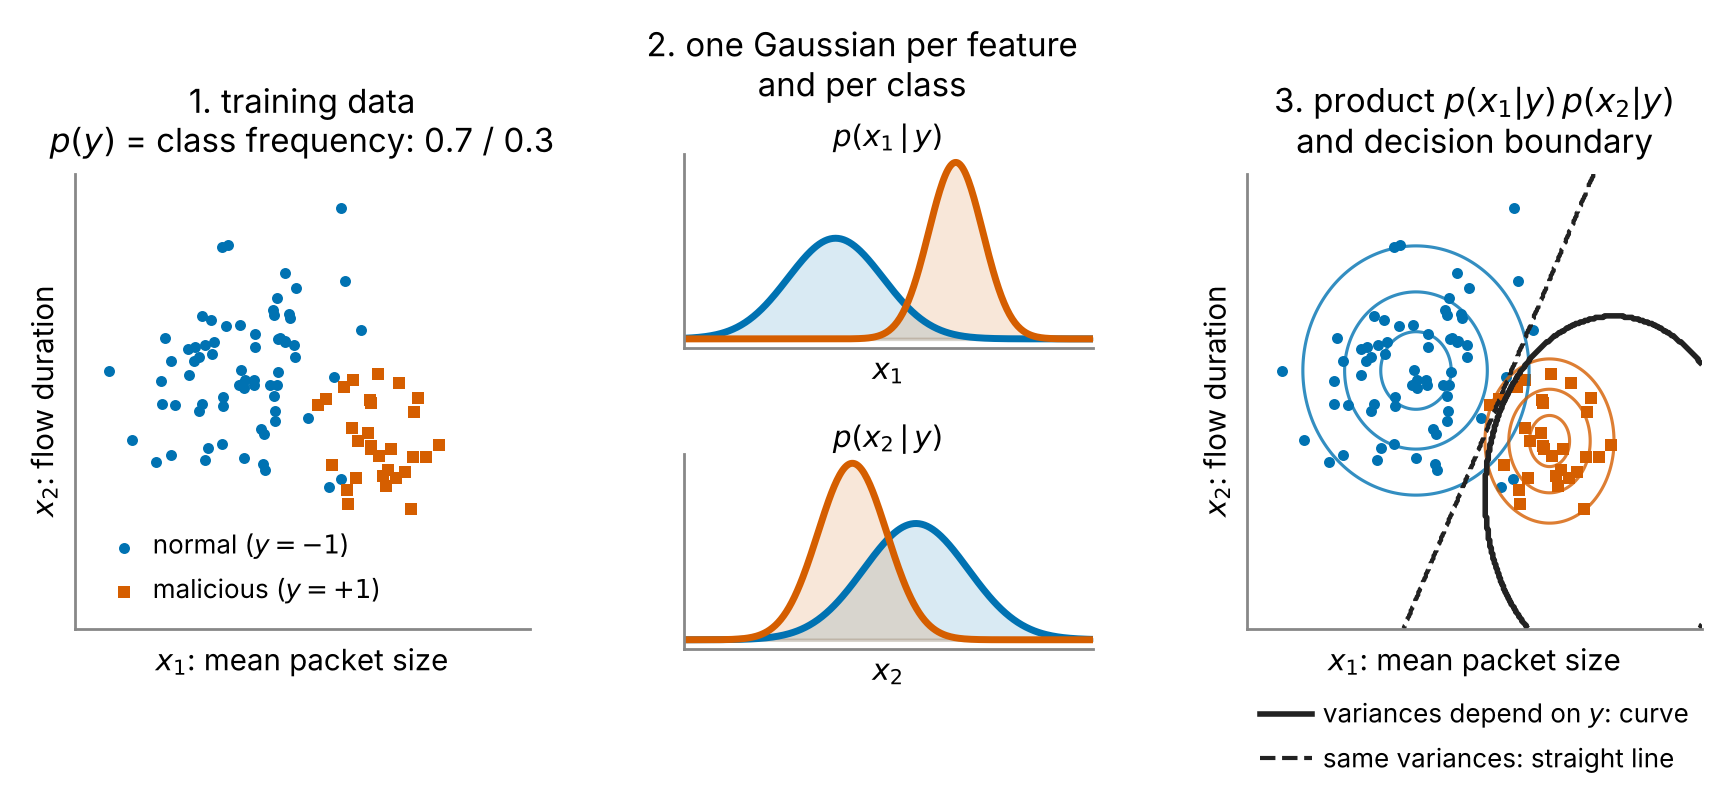
\includegraphics[width=1\textwidth]{images/chapter_9/naive_bayes.png}
    \caption{Naive Bayes step by step on 100 flows (70 normal, 30 malicious): class frequencies, one Gaussian per feature and per class, and their product with the resulting decision boundary.}
\end{figure}

For example, suppose that for a new flow the Gaussians give $p(x_1\,|\,\text{normal}) = 0.05$, $p(x_2\,|\,\text{normal}) = 0.30$, $p(x_1\,|\,\text{malicious}) = 0.40$ and $p(x_2\,|\,\text{malicious}) = 0.20$, with class frequencies $0.7$ and $0.3$. Then normal scores $0.7 \cdot 0.05 \cdot 0.30 = 0.0105$ and malicious scores $0.3 \cdot 0.40 \cdot 0.20 = 0.024$: the flow is classified as malicious, although normal flows are more frequent. The independence hypothesis is rarely true (packet size and throughput are correlated), but Naive Bayes works well in practice: it has only two parameters per feature and per class, it is extremely fast to train, and it needs little data.

\subsection{Decision Tree}
The \textbf{Decision Tree} has the following characteristics:
\begin{itemize}
    \item it is a \textbf{regressor and a classifier};
    \item \textbf{DATA}: numeric and categorical features, arbitrary label;
    \item \textbf{MODEL}: piecewise constant maps, represented by a flowchart, the decision tree;
    \item \textbf{LOSS}: different options for the loss function (e.g. Gini impurity or entropy for classification, squared error for regression), which are optimized locally and greedily, not globally.
\end{itemize}

\paragraph{Decision Tree as Classifier.} Decision Trees are models that use a tree-like structure containing only conditional control statements. A decision tree can be represented as a flowchart in which:
\begin{itemize}
    \item \textbf{internal nodes} are condition tests on an attribute;
    \item each \textbf{branch} represents an outcome of the condition test;
    \item each \textbf{leaf node} holds a class label.
\end{itemize}
To classify a record we start from the root and follow the branches given by its features until we reach a leaf.

\begin{figure}[h]
    \centering
    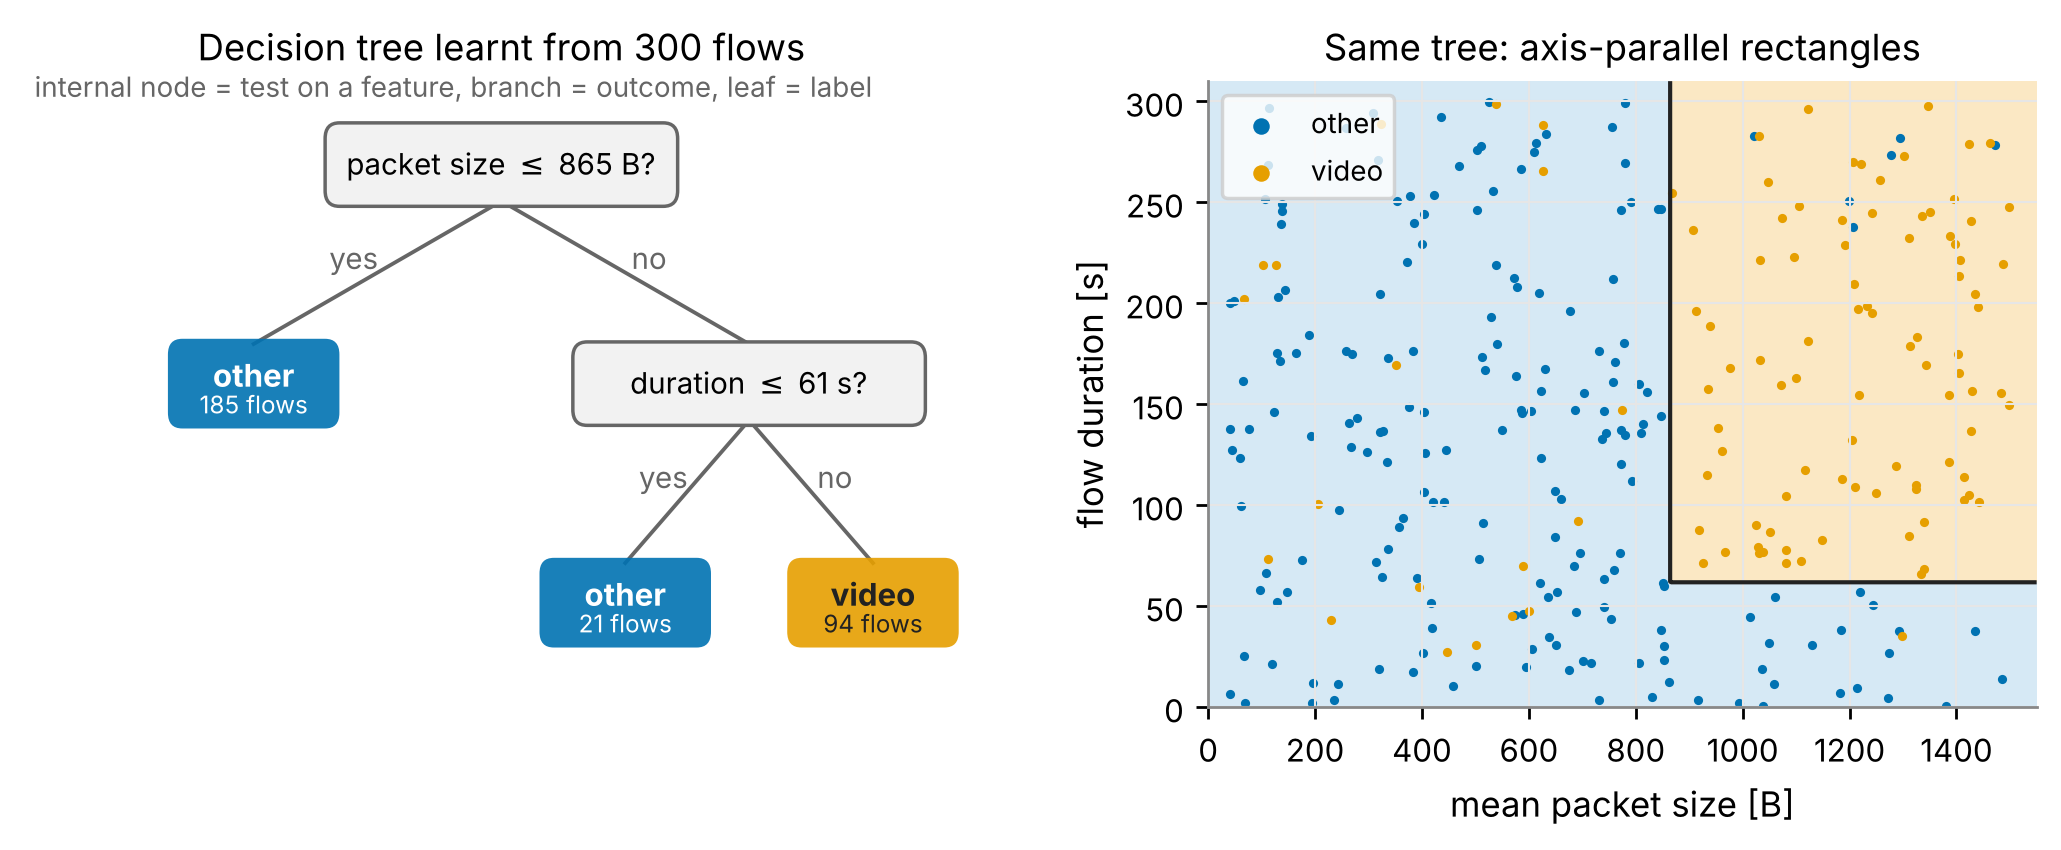
\includegraphics[width=1\textwidth]{images/chapter_9/decision_tree.png}
    \caption{Left: a decision tree that recognizes video flows, learnt from 300 flows. Right: the regions of the feature space defined by the same tree.}
\end{figure}

In the figure, a flow with mean packet size 1200 B and duration 120 s answers ``no'' to the first test and ``no'' to the second, so it is classified as video; with the same packet size and a duration of 30 s it would be classified as other. Since each test compares \emph{one} feature with a threshold, the tree splits the feature space into rectangles with sides parallel to the axes, each with its own label. The tree is learnt greedily, from the root to the leaves:

\begin{center}
\fbox{\parbox{0.9\textwidth}{
\textbf{Algorithm: growing a decision tree (greedy)}\\
\textbf{Input:} training set, loss (e.g. Gini impurity), stopping rule (e.g. maximum depth)\\
\textbf{Output:} decision tree
\begin{enumerate}
    \item Put all the training points in the root.
    \item For the current node, try every feature and every threshold, and choose the split that makes the two children as pure as possible (smallest loss).
    \item Repeat step 2 on each child, until the node is pure or the stopping rule is met.
    \item Each leaf predicts the majority class of its points (the mean label for regression).
\end{enumerate}}}
\end{center}
Each split is the best one \emph{now}, without looking ahead: finding the globally optimal tree would be computationally infeasible. The Decision Tree allows for non-linear decision boundaries, it is extremely fast at classifying unknown records (a handful of comparisons) and it is easy to interpret for small-sized trees. Its weak point is overfitting: a tree grown without limits ends up with a leaf for almost every training point, and small changes in the data can produce a very different tree. The maximum depth is its main hyper-parameter (see the validation curve in the previous chapter).

The Decision Tree for regression tasks works similarly to the one for classification, but in this case the output of each leaf is a single number, the average label of its training points. The prediction is therefore a staircase, a \textbf{piecewise constant} function.

\begin{figure}[h]
    \centering
    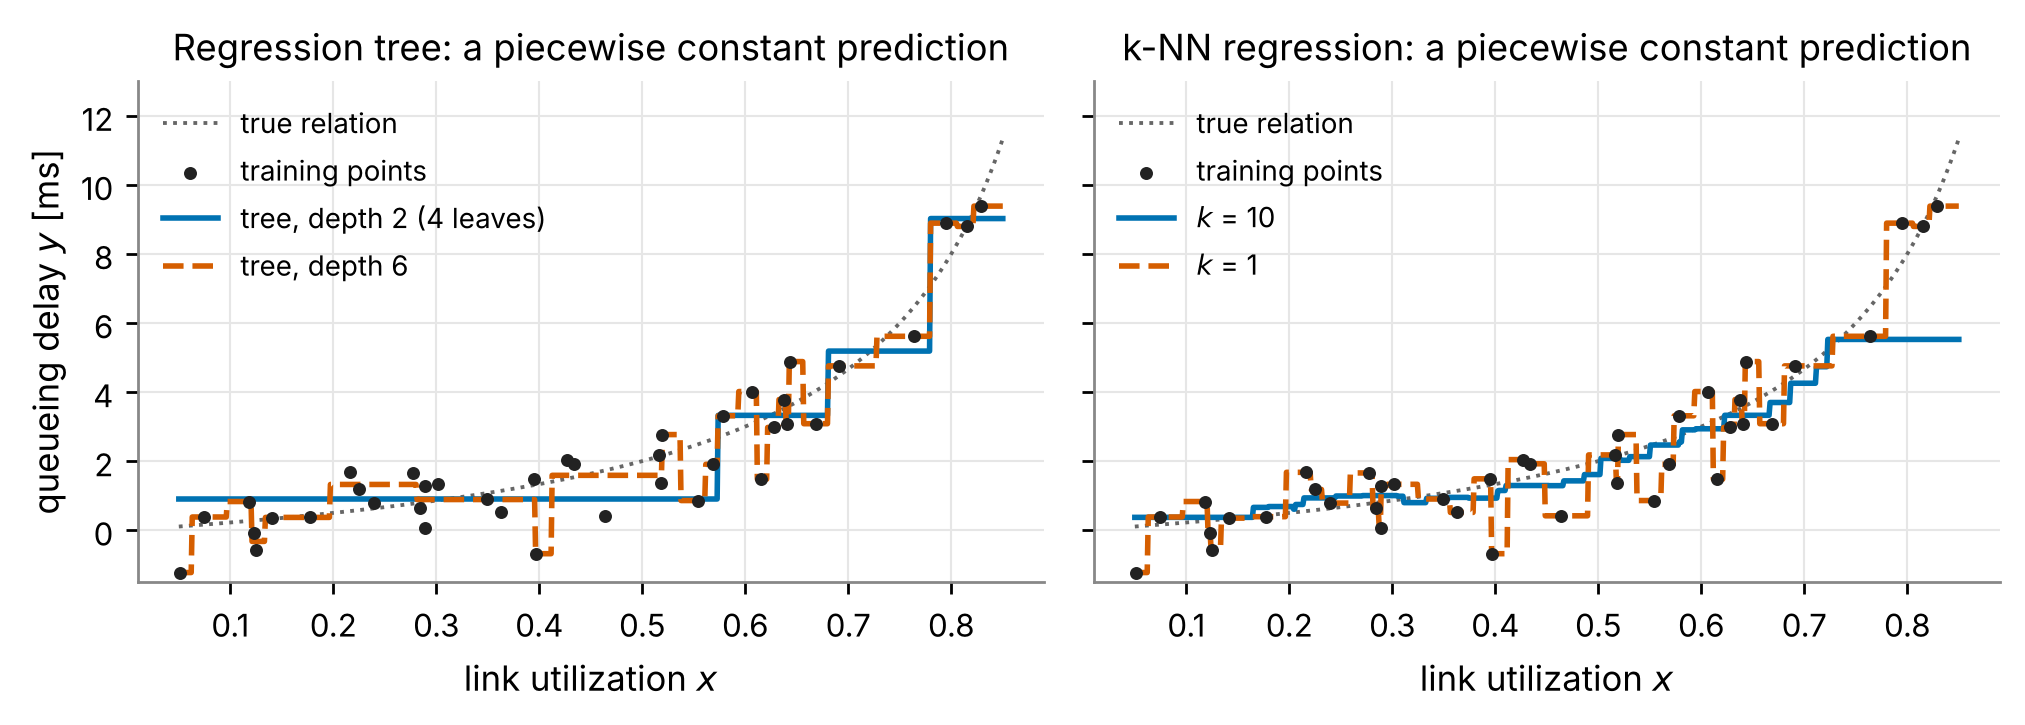
\includegraphics[width=1\textwidth]{images/chapter_9/piecewise_constant.png}
    \caption{Predicting the queueing delay of a link from its utilization (40 points). Regression trees and k-NN both give piecewise constant predictions; deep trees and $k = 1$ follow the noise.}
\end{figure}

\subsection{Random Forest}
The \textbf{Random Forest} is an ensemble classifier that consists of many decision trees, and it can also be used as an ensemble regressor. The RF outputs the class according to the results of the different trees, for instance by majority voting (by averaging their outputs for regression).\footnote{Correction: the previous version wrote ``DT outputs the class according to the results of the different trees''; it is the random forest (RF) that combines the trees.}

For each of the $K$ trees in the forest, a random subset of $n'$ features and a random subset of $m'$ training samples are selected. By changing the data we obtain different hypotheses. Then, looking at the results of the different hypotheses, the forest performs majority voting to determine the output.\footnote{Note: in the standard random forest (Breiman's algorithm, and RandomForestClassifier in scikit-learn) each tree is trained on a bootstrap sample, i.e. $m' = m$ points drawn \emph{with replacement}, and the random subset of $n'$ features is drawn again \emph{at each split}, not once per tree. The description above may follow the convention of the course; check the slides.}

\begin{center}
\fbox{\parbox{0.9\textwidth}{
\textbf{Algorithm: random forest}\\
\textbf{Input:} training set with $m$ points and $n$ features, number of trees $K$, sizes $m'$ and $n'$\\
\textbf{Output:} prediction for a new record $\mathbf{x}$
\begin{enumerate}
    \item For $k = 1, \dots, K$: draw $m'$ training points and $n'$ features at random, and grow tree $k$ on them.
    \item To predict $\mathbf{x}$, compute the output of every tree.
    \item Return the majority class (classification) or the average output (regression).
\end{enumerate}}}
\end{center}

A single deep tree has low bias but high variance: it changes a lot with the training data. Trees trained on different data make different errors, and the vote averages them out, like the ``wisdom of the crowd''. If each of 25 trees were right 70\% of the time and their errors were independent, the majority would be right about 98\% of the time. In reality the trees make correlated errors, and the random subsets of data and features are there precisely to make them as different as possible. The number of trees $K$ can be selected via the validation curve or set to a default number (100 in scikit-learn); the same goes for the number of features $n'$ (by default $\sqrt{n}$ for classification). More trees do not cause overfitting, they only cost more computation. The price is interpretability: a hundred trees cannot be read like a single small one.

\begin{figure}[h]
    \centering
    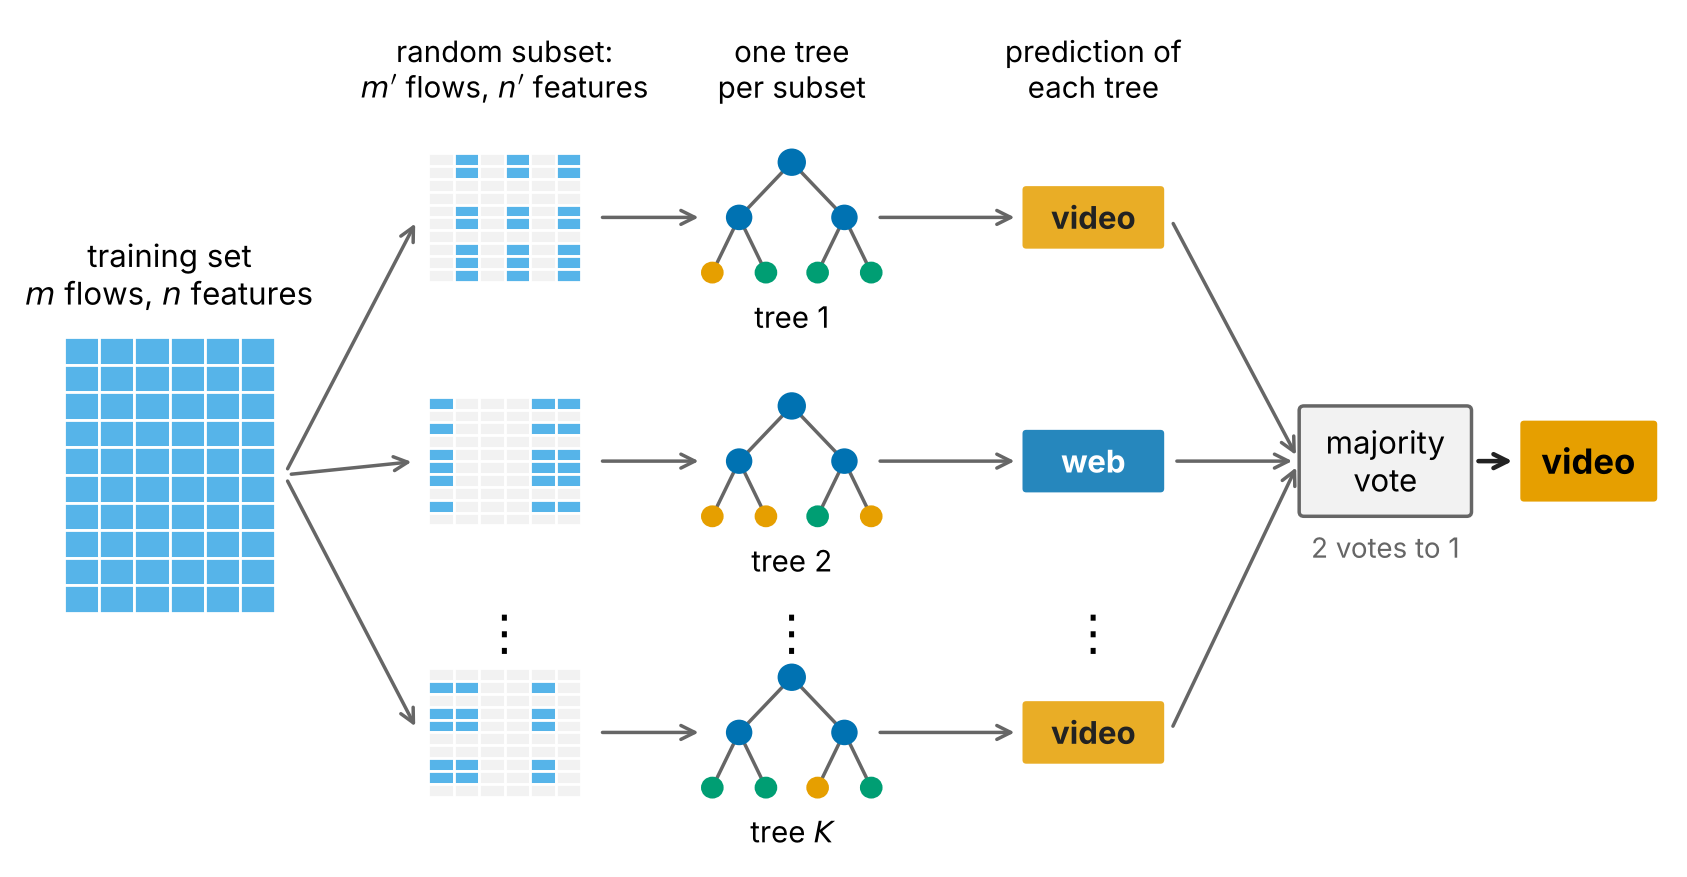
\includegraphics[width=0.95\textwidth]{images/chapter_9/random_forest.png}
    \caption{Random forest: each tree is trained on a random subset of flows and features, and the trees vote.}
\end{figure}

\subsection{k-Nearest Neighbors}
\textbf{k-NN} can be used to perform both supervised regression and classification tasks. It has the following properties:
\begin{itemize}
    \item \textbf{DATA}: numeric features, numeric or categorical label;
    \item \textbf{MODEL}: piecewise constant map; the hypothesis space of k-NN depends on the labelled dataset;
    \item \textbf{LOSS}: no loss function, since nothing is optimized and there is no training.
\end{itemize}
k-NN is an \textbf{instance-based} (or lazy) learning method, since it does not construct a general internal model. It simply stores the instances of the training data, and uses the $k$ closest points to perform the classification or the regression. As a classifier, k-NN requires:
\begin{itemize}
    \item the set of stored records;
    \item a distance metric to compute the distance between records, e.g. the Euclidean distance;
    \item the value of $k$.
\end{itemize}

\begin{center}
\fbox{\parbox{0.9\textwidth}{
\textbf{Algorithm: k-NN prediction}\\
\textbf{Input:} stored records with their labels, distance metric, $k$, unknown record $\mathbf{x}$\\
\textbf{Output:} predicted label of $\mathbf{x}$
\begin{enumerate}
    \item Compute the distance from $\mathbf{x}$ to every stored record.
    \item Identify the $k$ nearest neighbors.
    \item Classification: return the majority class of their labels. Regression: return the average of their labels.
\end{enumerate}}}
\end{center}

\begin{figure}[h]
    \centering
    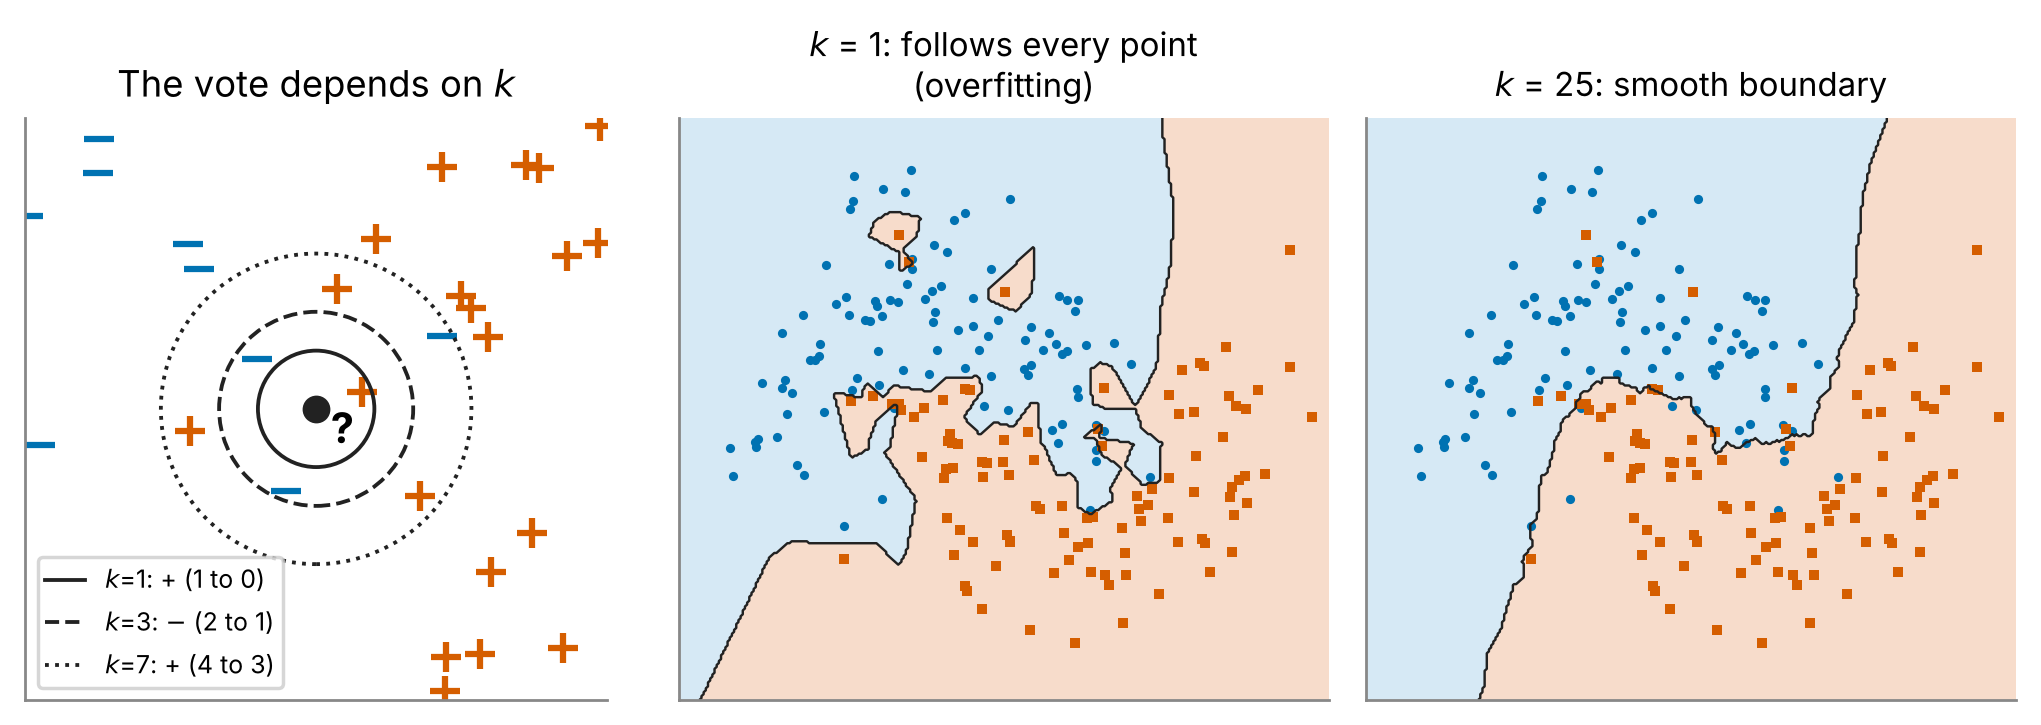
\includegraphics[width=1\textwidth]{images/chapter_9/knn.png}
    \caption{Left: the class of the unknown record changes with $k$. Centre and right: decision regions with $k = 1$ and $k = 25$.}
\end{figure}

In the figure, the unknown record is classified as $+$ with $k = 1$, as $-$ with $k = 3$ (two neighbours against one) and again as $+$ with $k = 7$ (four against three). For binary problems an odd $k$ avoids ties. If $k$ is too small, the model is too sensitive to noise points, hence it can lead to \textbf{overfitting}: with $k = 1$ every isolated point creates its own island. If $k$ is too large, the neighbourhood may include many points from other classes, and the boundary becomes too smooth (\textbf{underfitting}); with $k = m$ every record gets the majority class. Hence, it is recommended to perform validation in order to tune the best value of $k$. For regression, k-NN averages the labels of the $k$ neighbours, and its prediction is again piecewise constant (right panel of the piecewise constant figure above).

Lastly, before applying k-NN the attribute domains should be \textbf{normalized}, to prevent the distance from being dominated by one of the attributes. Two flows that differ by 30 s in duration and by 100\,000 bytes have a Euclidean distance of about 100\,000: the duration does not count at all, and the neighbours are chosen only by the number of bytes.

\begin{figure}[h]
    \centering
    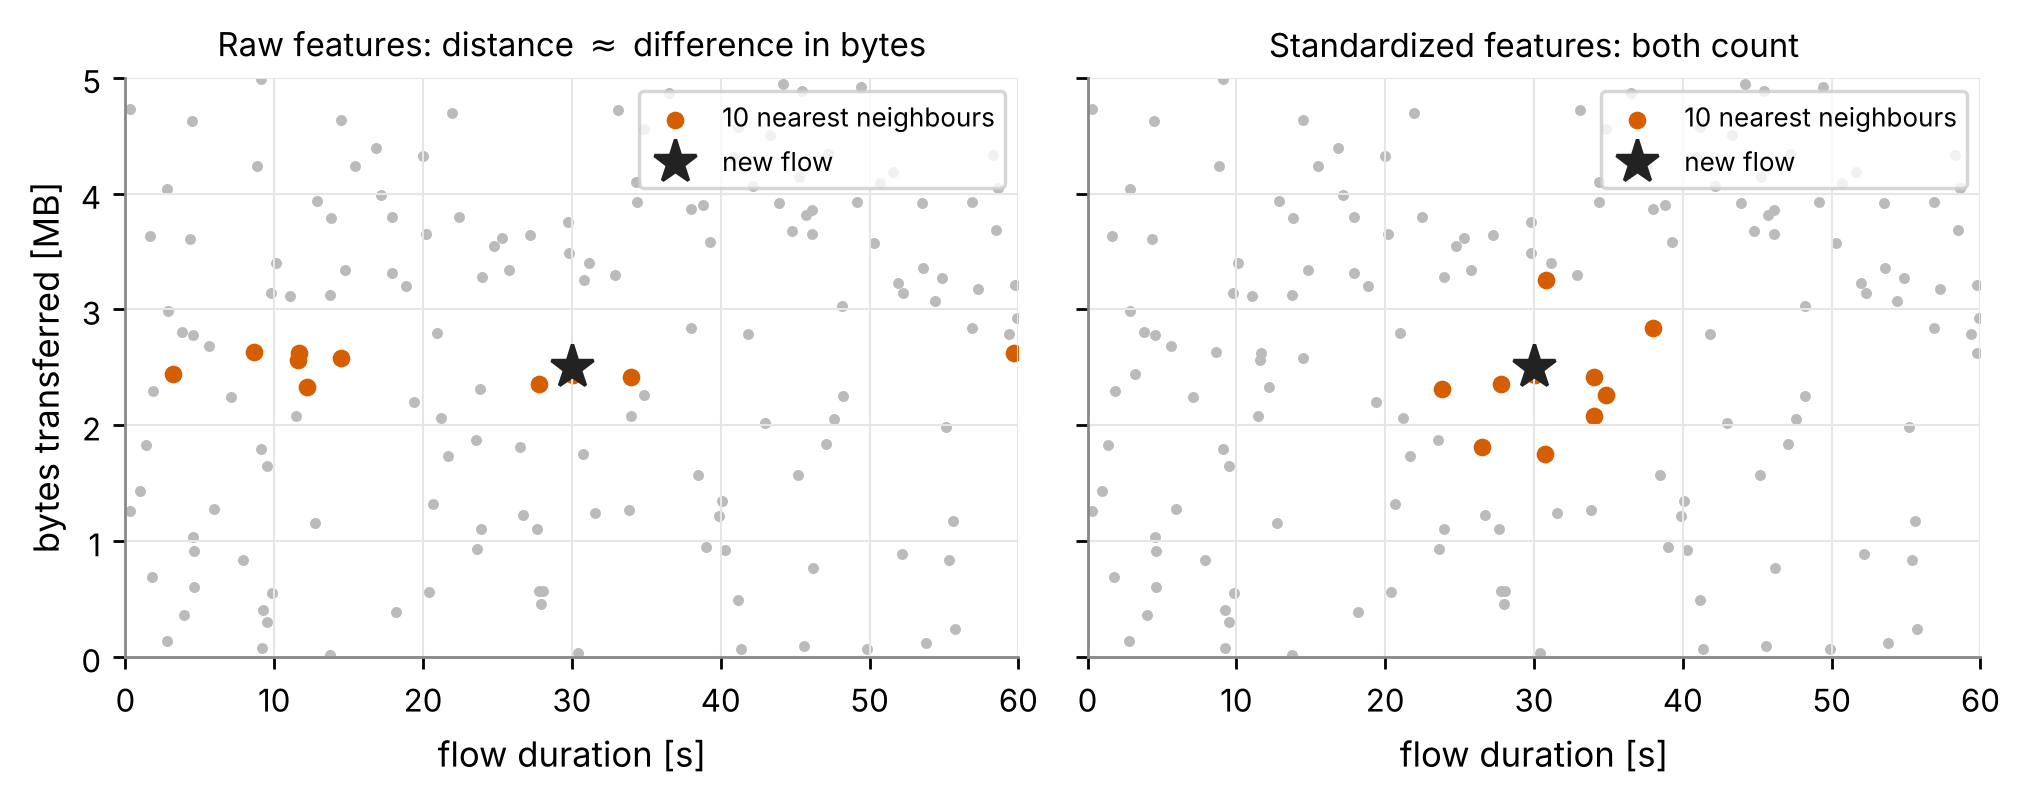
\includegraphics[width=1\textwidth]{images/chapter_9/knn_scaling.png}
    \caption{The 10 nearest neighbours of a new flow, with raw features (left) and standardized features (right).}
\end{figure}

k-NN has no training phase, but its predictions are slow: for each new record it computes the distance to \emph{all} the $m$ stored records, i.e. about $m \cdot n$ operations, whatever the value of $k$. With one million stored flows and 20 features, that is 20 million operations per prediction. It is also not very scalable, since it needs to store all the data points in memory.\footnote{Correction: the previous version said that k-NN ``is slow if k is really high''. The cost of a prediction is dominated by the distances to all the $m$ stored records, which must be computed for any $k$; choosing the $k$ smallest adds little.}

\subsection{Comparison}
The figure below applies six of the techniques to the same two-dimensional problem: two interleaved classes, as normal and anomalous traffic can be in a feature space, with 280 training and 120 test points.

\begin{figure}[h]
    \centering
    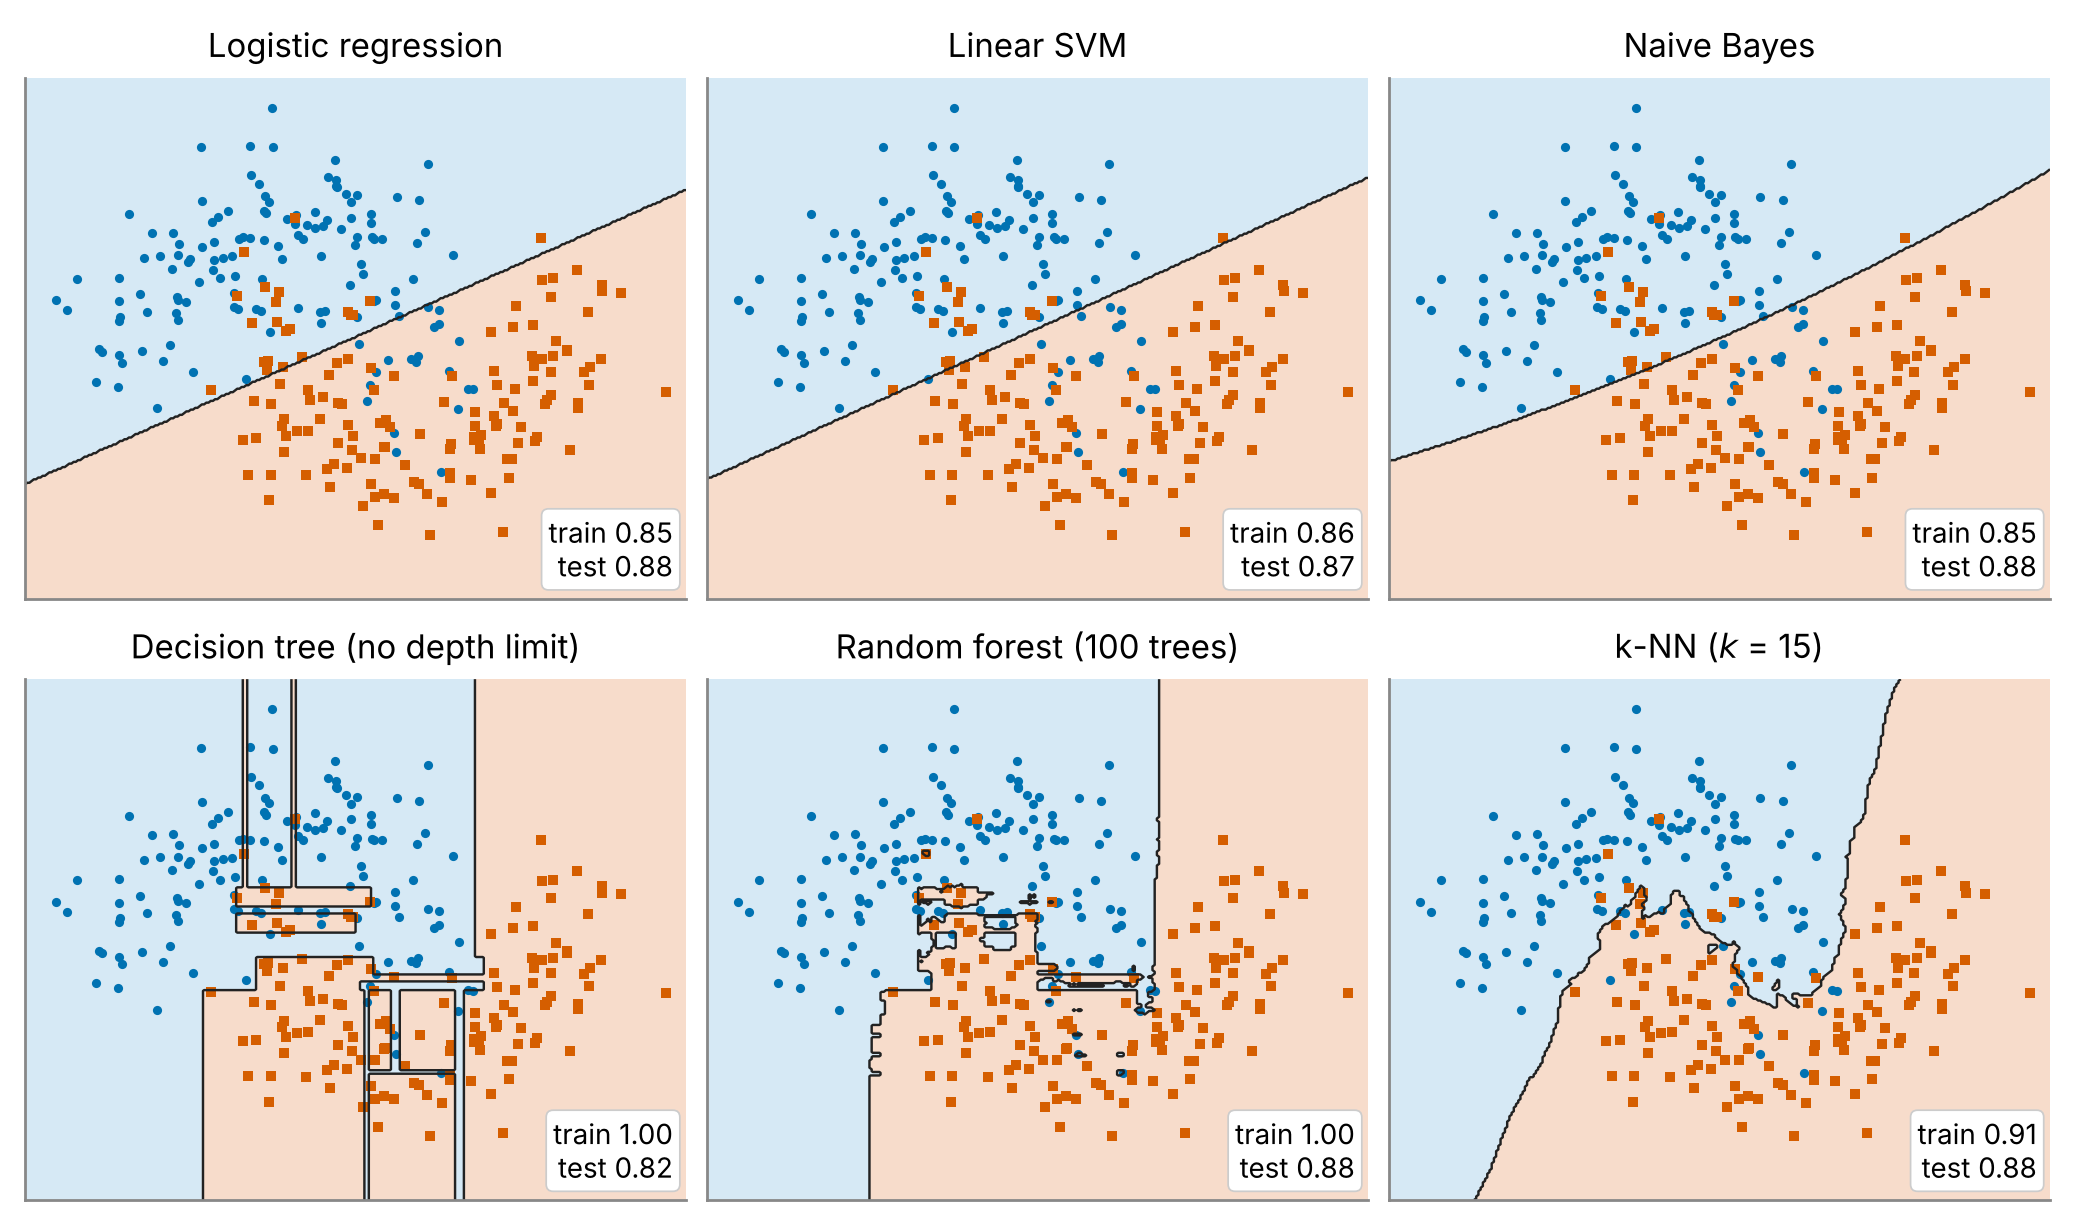
\includegraphics[width=1\textwidth]{images/chapter_9/boundaries_comparison.png}
    \caption{Decision regions of six classifiers on the same data, with training and test accuracy.}
\end{figure}

The linear methods (logistic regression, SVM and, almost, Naive Bayes) draw a straight line and reach a test accuracy of $0.87$--$0.88$. The decision tree grown without limits is perfect on the training set ($1.00$) but has the lowest test accuracy ($0.82$): it overfits with many small rectangles. The random forest smooths these rectangles and raises the test accuracy to $0.88$, and k-NN with $k = 15$ follows the curved shape of the classes. With 120 test points one error changes the accuracy by about $0.008$, so differences of $0.01$ should not be over-interpreted.

\begin{center}
    \begin{tabular}{l|l|l|l}
        \textbf{Method} & \textbf{Task} & \textbf{Model} & \textbf{Loss} \\ \hline
        Linear regression   & R    & linear maps        & squared error \\
        LASSO               & R    & linear maps        & squared error $+\ \lambda\|\mathbf{w}\|_1$ \\
        Logistic regression & C    & linear maps        & logistic loss \\
        SVM                 & C    & linear maps        & hinge loss $+\ \lambda\|\mathbf{w}\|_2^2$ \\
        Naive Bayes         & C    & linear maps        & 0/1 loss (Bayes' rule) \\
        Decision tree       & R, C & piecewise constant & impurity, greedy \\
        Random forest       & R, C & vote of trees      & impurity, per tree \\
        k-NN                & R, C & piecewise constant & none \\
    \end{tabular}
\end{center}
(R = regression, C = classification.)

\section{Summary}
\begin{itemize}
    \item \textbf{Gradient descent} minimizes the empirical risk by repeated steps $\mathbf{w}^{(r+1)} = \mathbf{w}^{(r)} - \alpha\nabla f(\mathbf{w}^{(r)})$, against the gradient.
    \item The \textbf{learning rate} must be neither too small (slow) nor too large (divergence); standardized features need fewer steps. GD stops after a fixed number of epochs, when the risk stops improving, or when the validation error stops decreasing (early stopping).
    \item \textbf{SGD} estimates the gradient on one random point or on a random batch: cheap, noisy steps, suited to large datasets.
    \item \textbf{Multi-class}: one-vs-rest (one binary problem per class) or softmax with cross-entropy loss. \textbf{Multi-label}: one problem per label, or one class per combination of labels.
    \item \textbf{LASSO}: linear regression with an L1 penalty that sets weights to zero (feature selection). \textbf{SVM}: linear classifier with the maximum margin (regularized hinge loss). \textbf{Naive Bayes}: Bayes classifier with independent Gaussian features.
    \item \textbf{Decision trees}: sequences of tests on single features, learnt greedily; \textbf{random forests}: many trees on random subsets, combined by voting; \textbf{k-NN}: vote of the $k$ nearest stored records, with normalized features.
\end{itemize}



\section{A prova di coglione}
Questo capitolo ha due anime. La prima risponde alla domanda ``come si minimizza davvero il rischio empirico?'': scendendo a piccoli passi, con il gradient descent. La seconda è un catalogo dei metodi supervisionati più usati, ognuno descritto con la solita ricetta dell'ERM (dati, modello, loss): conoscere bene quella ricetta vuol dire avere già metà del capitolo in tasca.

\subsection{Gradient descent: scendere a piccoli passi}
\paragraph*{L'idea.} Sei in montagna nella nebbia e vuoi arrivare a valle. La valle non la vedi, ma senti la pendenza sotto i piedi: fai un passo in discesa, poi un altro, finché il terreno non diventa piatto.

Il gradiente è la pendenza e punta in \emph{salita}, quindi ci si muove dalla parte opposta: $\mathbf{w} \leftarrow \mathbf{w} - \alpha\nabla f(\mathbf{w})$. Il learning rate $\alpha$ è la lunghezza del passo. Troppo piccolo e non arrivi mai, troppo grande e salti da un versante all'altro della valle fino a scappare via. Su $f(w) = w^2$, partendo da $w = -4$: con $\alpha = 0.35$ ogni passo moltiplica $w$ per $0.3$ e in pochi passi sei al minimo; con $\alpha = 1.05$ lo moltiplica per $-1.1$ e diverge. Standardizzare le feature rende la valle più rotonda: nell'esempio del capitolo bastano 5 passi invece di 39.

Ci si ferma dopo un numero fisso di epoche, quando il rischio empirico smette di migliorare, oppure quando il \emph{validation} error smette di scendere (early stopping). Nell'esempio il punto giusto è l'epoca 64: continuare porta il validation error da $0.73$ a $30$, perché il modello impara il rumore.

Con milioni di dati, calcolare il gradiente esatto a ogni passo costa troppo. La \textbf{SGD} lo stima con la media su un solo punto, o su un piccolo batch, preso a caso. È come chiedere la strada a pochi passanti invece che a tutta la città: la risposta è più rumorosa, ma arriva subito. Con lo stesso lavoro di un solo passo di GD, nell'esempio la SGD è già a $0.42$ (minimo $0.40$), mentre il GD è ancora a $7.91$.

\begin{figure}[h]
    \centering
    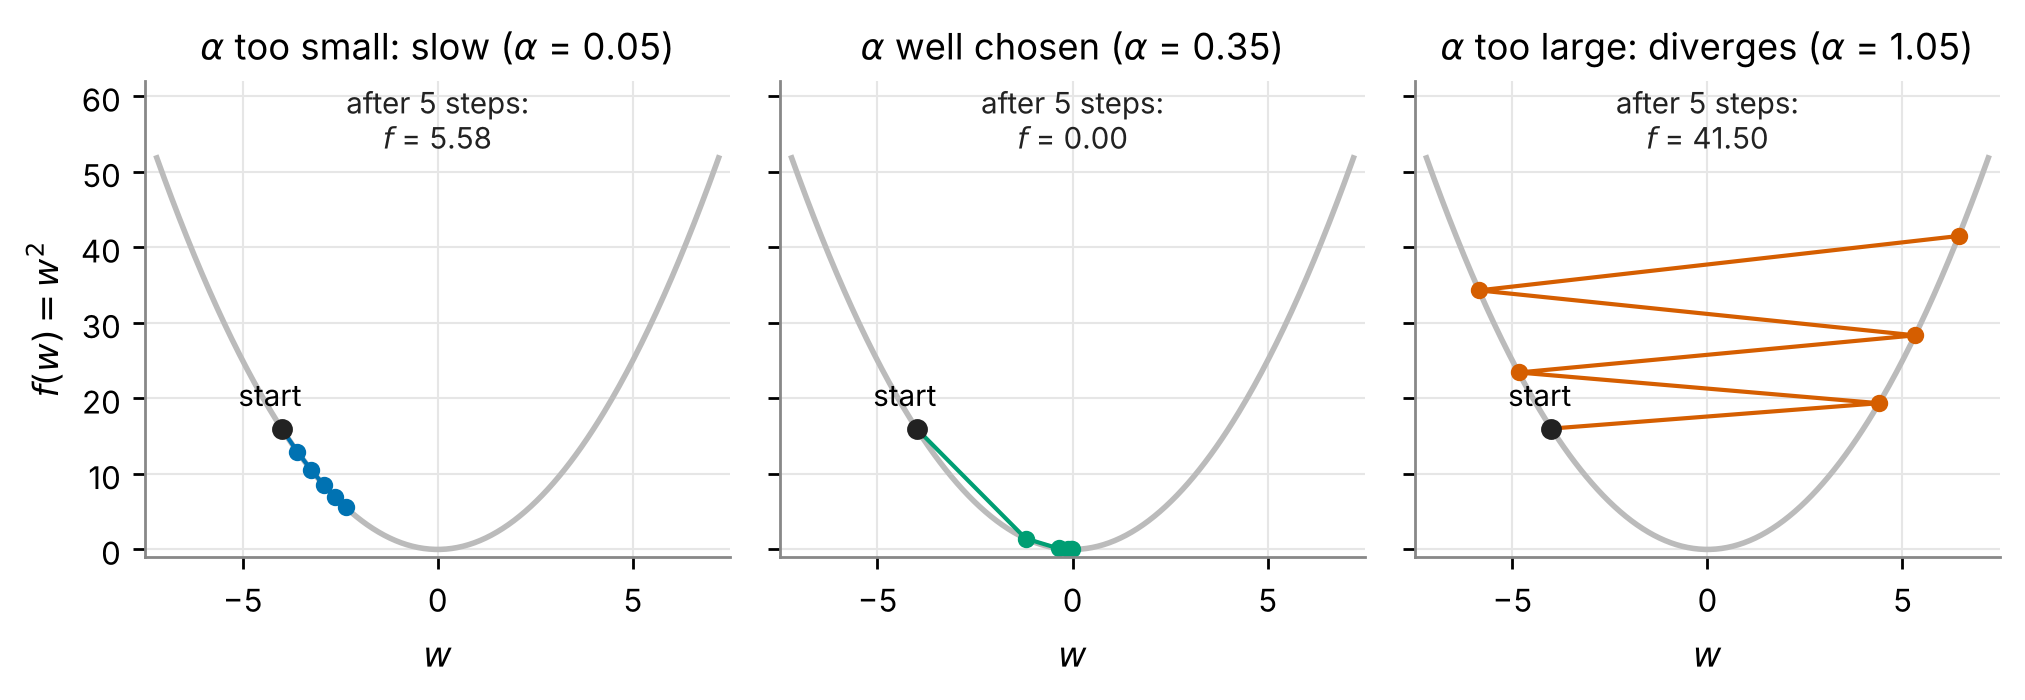
\includegraphics[width=1\textwidth]{images/chapter_9/learning_rate.png}
    \caption{Cinque passi di gradient descent su $f(w) = w^2$: learning rate troppo piccolo, giusto, troppo grande.}
\end{figure}

\subsection{Più di due classi}
\paragraph*{L'idea.} Con più classi ci sono due strade: spezzare il problema in tanti problemi binari, oppure trasformare i punteggi in probabilità.

Il \textbf{one-vs-rest} addestra un classificatore per classe (``è web o no?'', ``è video o no?'', ``è VoIP o no?'') e sceglie la classe con il punteggio più alto. La \textbf{softmax} dà un punteggio a ogni classe e lo trasforma in una probabilità, con somma 1; la loss è $-\log$ della probabilità data alla classe vera. Esempio: i punteggi $2$, $1$, $-1$ diventano $0.71$, $0.26$, $0.04$. Se la classe vera è web la loss è $0.35$; se è VoIP è $3.35$, perché il modello era sicuro e ha sbagliato.

Il \textbf{multi-label} è un'altra cosa: lo stesso dato ha più etichette, per esempio applicazione e cifrato sì/no. Si può addestrare un classificatore per ogni etichetta, oppure creare una classe per ogni combinazione ($3 \times 2 = 6$ classi).

\subsection{I metodi lineari: LASSO, SVM, Naive Bayes}
\paragraph*{L'idea.} Tre metodi con lo stesso modello, una retta (o un iperpiano), ma con un'idea diversa di ``retta migliore''.

\textbf{LASSO} è la regressione lineare con una multa $\lambda$ sulla somma dei $|w_j|$. La multa spinge a zero i pesi delle feature inutili: è una selezione automatica delle feature, e funziona anche quando ci sono più feature che dati. Nell'esempio sul throughput TCP, con il $\lambda$ scelto in cross validation 4 pesi su 10 diventano esattamente zero, e le 3 feature importanti (RTT, loss rate, utilizzo del link) restano quelle con i pesi più grandi.

La \textbf{SVM}, tra tutte le rette che separano le classi, sceglie quella con il margine più largo, la più lontana dai punti più vicini: è la strada più larga che si riesce a far passare tra le due classi. Con $\lambda$ più grande la strada si allarga, ma qualche punto può finirci dentro.

Il \textbf{Naive Bayes} non ottimizza niente. Stima dai dati quanto è frequente ogni classe e, per ogni feature, una gaussiana per classe; poi sceglie la classe più probabile. È ``naive'' perché fa finta che le feature siano indipendenti. Esempio: normale vale $0.7 \cdot 0.05 \cdot 0.30 = 0.0105$, malevolo vale $0.3 \cdot 0.40 \cdot 0.20 = 0.024$, quindi il flusso è malevolo, anche se i flussi normali sono più frequenti.

\subsection{I metodi non lineari: alberi, foreste, k-NN}
\paragraph*{L'idea.} Quando il confine tra le classi non è una retta servono modelli che dividono lo spazio in pezzi e danno una risposta costante in ogni pezzo.

Il \textbf{decision tree} è una serie di domande sì/no, come nel gioco ``Indovina chi?'': ``pacchetti più grandi di 865 byte? durata oltre 61 secondi? allora è video''. È velocissimo e si legge facilmente, ma se lo lasci crescere senza limiti impara a memoria (nel confronto finale: training $1.00$, test $0.82$).

La \textbf{random forest} sono tanti alberi, ognuno addestrato su un pezzo diverso di dati e di feature, che poi votano. Un albero da solo sbaglia spesso, la maggioranza molto meno: è la saggezza della folla. Nell'esempio il test sale da $0.82$ a $0.88$.

Il \textbf{k-NN} segue il proverbio ``dimmi con chi vai e ti dirò chi sei'': il nuovo dato prende la classe della maggioranza dei suoi $k$ vicini. Non c'è training, ma ogni previsione confronta il dato con \emph{tutti} quelli salvati. $k$ piccolo porta overfitting, $k$ grande underfitting. Le feature vanno normalizzate, altrimenti la distanza la decide solo quella con i numeri più grandi: i byte schiacciano i secondi.

\begin{figure}[h]
    \centering
    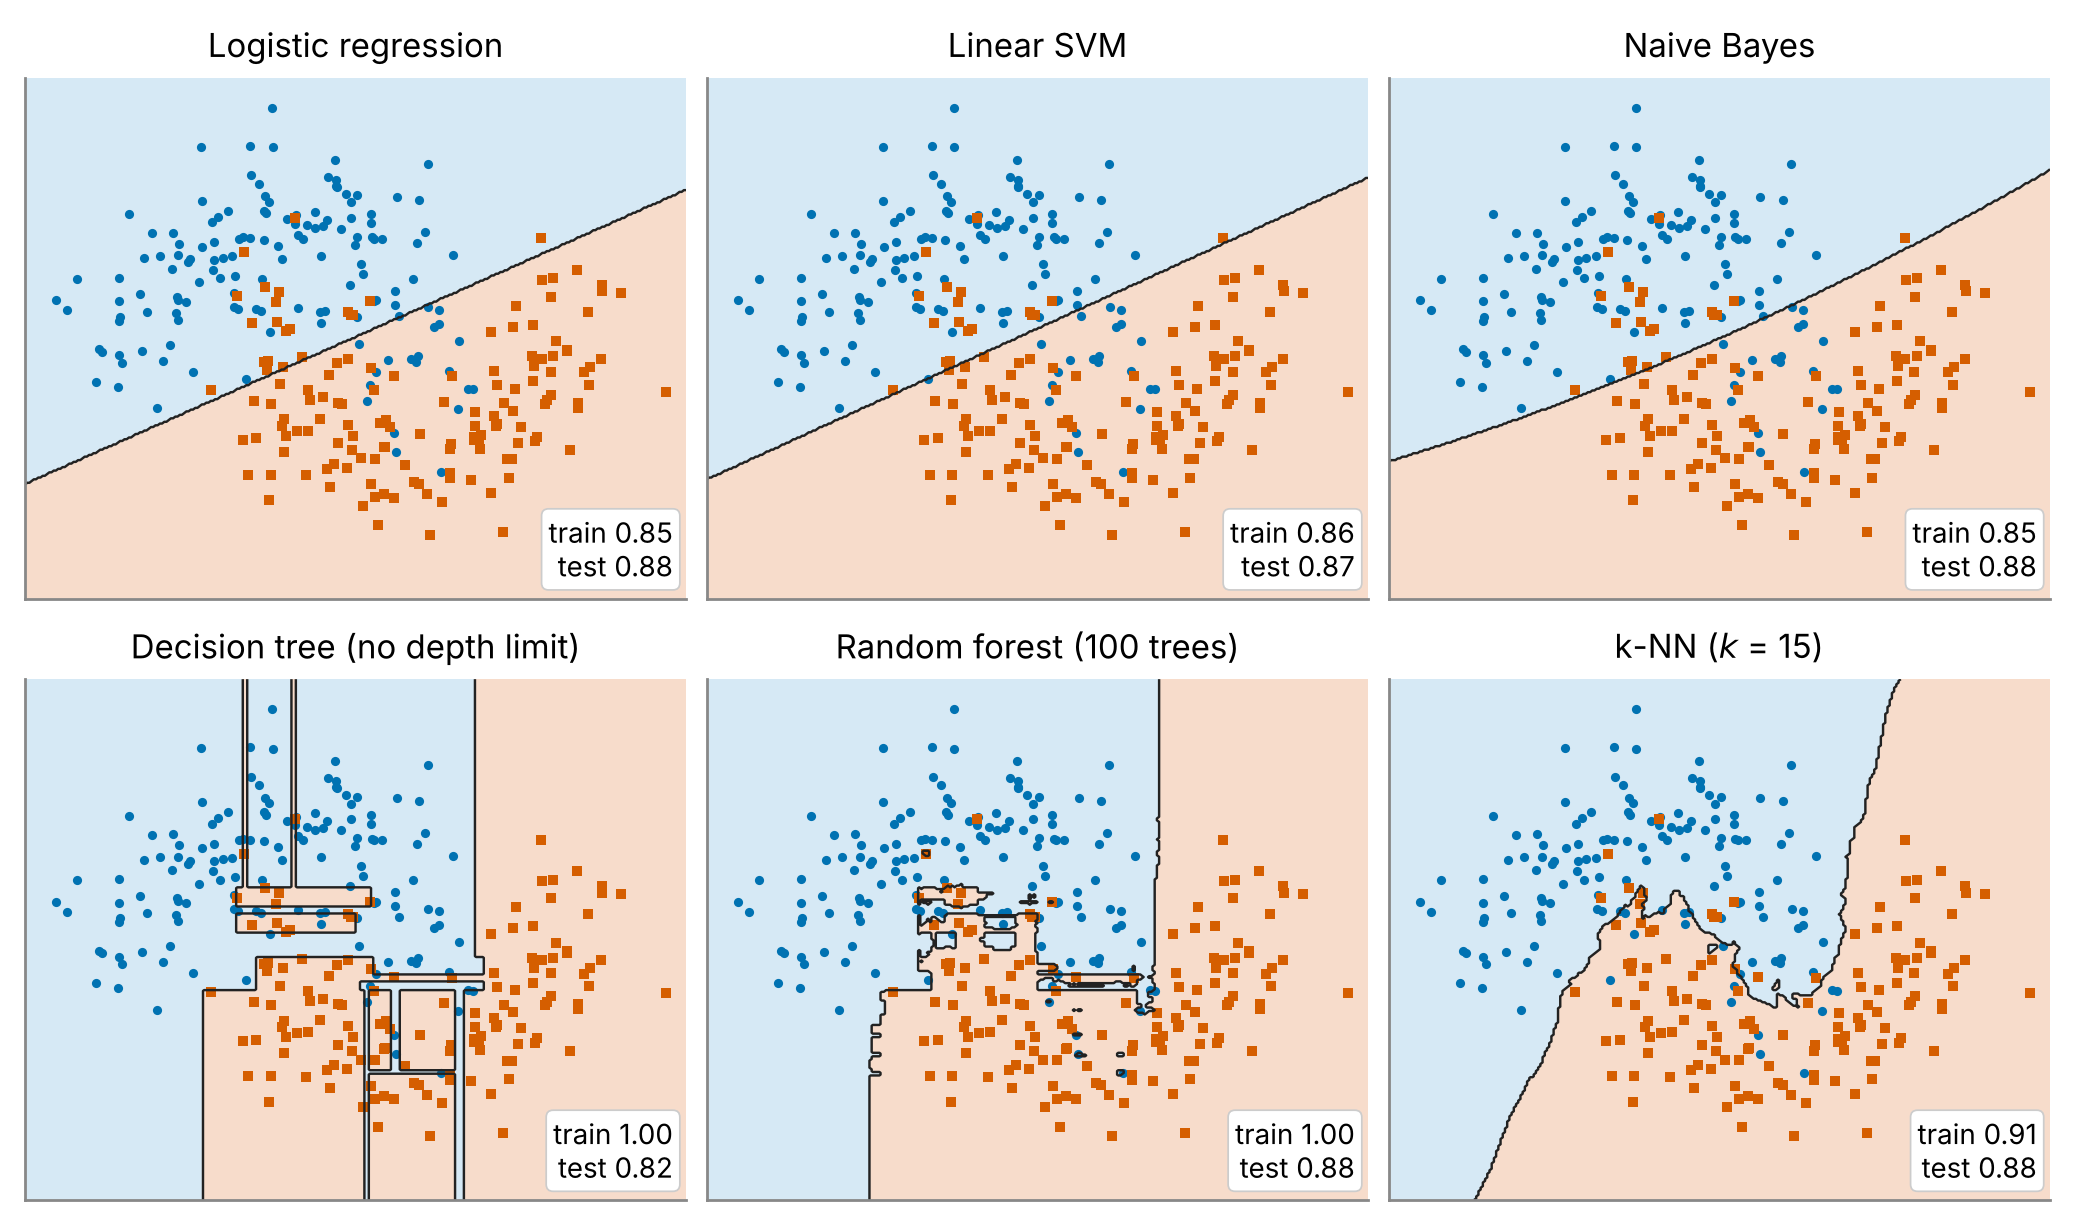
\includegraphics[width=0.8\textwidth]{images/chapter_9/boundaries_comparison.png}
    \caption{Sei metodi sugli stessi dati: i lineari tracciano una retta, l'albero fa rettangoli e va in overfitting, foresta e k-NN seguono la forma curva delle classi.}
\end{figure}

\subsection{Quando usare cosa}
\begin{center}
    \begin{tabular}{l|l}
        \textbf{Situazione} & \textbf{Metodo} \\ \hline
        Tante feature, poche davvero utili           & LASSO \\
        Classi separabili da una retta               & SVM, regressione logistica \\
        Pochi dati, serve qualcosa di veloce          & Naive Bayes \\
        Bisogna spiegare la decisione                 & albero poco profondo \\
        Accuratezza alta su dati tabellari            & random forest \\
        Confine irregolare, pochi dati e feature      & k-NN \\
        Moltissimi dati, aggiornamento continuo       & modelli addestrati con SGD \\
    \end{tabular}
\end{center}

\subsection{Da sapere per l'esame}
\begin{center}
    \begin{tabular}{l|l}
        \textbf{Concetto} & \textbf{In una riga} \\ \hline
        Gradient descent  & $\mathbf{w} \leftarrow \mathbf{w} - \alpha\nabla f(\mathbf{w})$: passo contro il gradiente \\ \hline
        Learning rate     & troppo piccolo: lento; troppo grande: diverge \\ \hline
        Standardizzazione & valle più rotonda, meno passi \\ \hline
        Quando fermarsi   & epoche fisse, rischio fermo, early stopping \\ \hline
        SGD               & gradiente stimato con la media su un punto o un batch \\ \hline
        One-vs-rest       & un problema binario per classe, vince lo score più alto \\ \hline
        Softmax           & punteggi $\rightarrow$ probabilità; loss $= -\log p(\text{classe vera})$ \\ \hline
        Multi-label       & un modello per etichetta, o una classe per combinazione \\ \hline
        LASSO             & squared loss $+\ \lambda\|\mathbf{w}\|_1$: pesi a zero, selezione feature \\ \hline
        SVM               & hinge loss $+\ \lambda\|\mathbf{w}\|_2^2$: margine massimo \\ \hline
        Naive Bayes       & classe con $p(\mathbf{x}|y)\,p(y)$ massimo, feature indipendenti \\ \hline
        Decision tree     & domande su una feature alla volta, costruzione greedy \\ \hline
        Random forest     & $K$ alberi su dati e feature diversi, voto di maggioranza \\ \hline
        k-NN              & voto dei $k$ vicini; niente training, feature normalizzate \\
    \end{tabular}
\end{center}
